\documentclass[twoside]{book}

% Packages required by doxygen
\usepackage{calc}
\usepackage{doxygen}
\usepackage{graphicx}
\usepackage[utf8]{inputenc}
\usepackage{makeidx}
\usepackage{multicol}
\usepackage{multirow}
\usepackage{textcomp}
\usepackage[table]{xcolor}

% Font selection
\usepackage[T1]{fontenc}
\usepackage{mathptmx}
\usepackage[scaled=.90]{helvet}
\usepackage{courier}
\usepackage{amssymb}
\usepackage{sectsty}
\renewcommand{\familydefault}{\sfdefault}
\allsectionsfont{%
  \fontseries{bc}\selectfont%
  \color{darkgray}%
}
\renewcommand{\DoxyLabelFont}{%
  \fontseries{bc}\selectfont%
  \color{darkgray}%
}

% Page & text layout
\usepackage{geometry}
\geometry{%
  a4paper,%
  top=2.5cm,%
  bottom=2.5cm,%
  left=2.5cm,%
  right=2.5cm%
}
\tolerance=750
\hfuzz=15pt
\hbadness=750
\setlength{\emergencystretch}{15pt}
\setlength{\parindent}{0cm}
\setlength{\parskip}{0.2cm}
\makeatletter
\renewcommand{\paragraph}{%
  \@startsection{paragraph}{4}{0ex}{-1.0ex}{1.0ex}{%
    \normalfont\normalsize\bfseries\SS@parafont%
  }%
}
\renewcommand{\subparagraph}{%
  \@startsection{subparagraph}{5}{0ex}{-1.0ex}{1.0ex}{%
    \normalfont\normalsize\bfseries\SS@subparafont%
  }%
}
\makeatother

% Headers & footers
\usepackage{fancyhdr}
\pagestyle{fancyplain}
\fancyhead[LE]{\fancyplain{}{\bfseries\thepage}}
\fancyhead[CE]{\fancyplain{}{}}
\fancyhead[RE]{\fancyplain{}{\bfseries\leftmark}}
\fancyhead[LO]{\fancyplain{}{\bfseries\rightmark}}
\fancyhead[CO]{\fancyplain{}{}}
\fancyhead[RO]{\fancyplain{}{\bfseries\thepage}}
\fancyfoot[LE]{\fancyplain{}{}}
\fancyfoot[CE]{\fancyplain{}{}}
\fancyfoot[RE]{\fancyplain{}{\bfseries\scriptsize Generated on Sat Feb 20 2016 14\-:23\-:47 for Trabalho\-\_\-de\-\_\-\-Grafos by Doxygen }}
\fancyfoot[LO]{\fancyplain{}{\bfseries\scriptsize Generated on Sat Feb 20 2016 14\-:23\-:47 for Trabalho\-\_\-de\-\_\-\-Grafos by Doxygen }}
\fancyfoot[CO]{\fancyplain{}{}}
\fancyfoot[RO]{\fancyplain{}{}}
\renewcommand{\footrulewidth}{0.4pt}
\renewcommand{\chaptermark}[1]{%
  \markboth{#1}{}%
}
\renewcommand{\sectionmark}[1]{%
  \markright{\thesection\ #1}%
}

% Indices & bibliography
\usepackage{natbib}
\usepackage[titles]{tocloft}
\setcounter{tocdepth}{3}
\setcounter{secnumdepth}{5}
\makeindex

% Hyperlinks (required, but should be loaded last)
\usepackage{ifpdf}
\ifpdf
  \usepackage[pdftex,pagebackref=true]{hyperref}
\else
  \usepackage[ps2pdf,pagebackref=true]{hyperref}
\fi
\hypersetup{%
  colorlinks=true,%
  linkcolor=blue,%
  citecolor=blue,%
  unicode%
}

% Custom commands
\newcommand{\clearemptydoublepage}{%
  \newpage{\pagestyle{empty}\cleardoublepage}%
}


%===== C O N T E N T S =====

\begin{document}

% Titlepage & ToC
\hypersetup{pageanchor=false}
\pagenumbering{roman}
\begin{titlepage}
\vspace*{7cm}
\begin{center}%
{\Large Trabalho\-\_\-de\-\_\-\-Grafos }\\
\vspace*{1cm}
{\large Generated by Doxygen 1.8.6}\\
\vspace*{0.5cm}
{\small Sat Feb 20 2016 14:23:47}\\
\end{center}
\end{titlepage}
\clearemptydoublepage
\tableofcontents
\clearemptydoublepage
\pagenumbering{arabic}
\hypersetup{pageanchor=true}

%--- Begin generated contents ---
\chapter{Hierarchical Index}
\section{Class Hierarchy}
This inheritance list is sorted roughly, but not completely, alphabetically\-:\begin{DoxyCompactList}
\item \contentsline{section}{Item}{\pageref{class_item}}{}
\begin{DoxyCompactList}
\item \contentsline{section}{Aresta}{\pageref{class_aresta}}{}
\item \contentsline{section}{Vertice}{\pageref{class_vertice}}{}
\end{DoxyCompactList}
\item \contentsline{section}{Leitura\-Gravacao}{\pageref{class_leitura_gravacao}}{}
\item \contentsline{section}{Lista}{\pageref{class_lista}}{}
\begin{DoxyCompactList}
\item \contentsline{section}{Grafo}{\pageref{class_grafo}}{}
\item \contentsline{section}{Vertice}{\pageref{class_vertice}}{}
\end{DoxyCompactList}
\end{DoxyCompactList}

\chapter{Class Index}
\section{Class List}
Here are the classes, structs, unions and interfaces with brief descriptions\-:\begin{DoxyCompactList}
\item\contentsline{section}{\hyperlink{class_aresta}{Aresta} }{\pageref{class_aresta}}{}
\item\contentsline{section}{\hyperlink{class_grafo}{Grafo} }{\pageref{class_grafo}}{}
\item\contentsline{section}{\hyperlink{class_item}{Item} }{\pageref{class_item}}{}
\item\contentsline{section}{\hyperlink{class_leitura_gravacao}{Leitura\-Gravacao} }{\pageref{class_leitura_gravacao}}{}
\item\contentsline{section}{\hyperlink{class_lista}{Lista} }{\pageref{class_lista}}{}
\item\contentsline{section}{\hyperlink{class_vertice}{Vertice} }{\pageref{class_vertice}}{}
\end{DoxyCompactList}

\chapter{File Index}
\section{File List}
Here is a list of all files with brief descriptions\-:\begin{DoxyCompactList}
\item\contentsline{section}{\hyperlink{_grafo_8cpp}{Grafo.\-cpp} }{\pageref{_grafo_8cpp}}{}
\item\contentsline{section}{\hyperlink{_grafo_8h}{Grafo.\-h} }{\pageref{_grafo_8h}}{}
\item\contentsline{section}{\hyperlink{_leitura_gravacao_8cpp}{Leitura\-Gravacao.\-cpp} }{\pageref{_leitura_gravacao_8cpp}}{}
\item\contentsline{section}{\hyperlink{_leitura_gravacao_8h}{Leitura\-Gravacao.\-h} }{\pageref{_leitura_gravacao_8h}}{}
\item\contentsline{section}{\hyperlink{_lista_8cpp}{Lista.\-cpp} }{\pageref{_lista_8cpp}}{}
\item\contentsline{section}{\hyperlink{_lista_8h}{Lista.\-h} }{\pageref{_lista_8h}}{}
\item\contentsline{section}{\hyperlink{main_8cpp}{main.\-cpp} }{\pageref{main_8cpp}}{}
\end{DoxyCompactList}

\chapter{Class Documentation}
\hypertarget{class_aresta}{\section{Aresta Class Reference}
\label{class_aresta}\index{Aresta@{Aresta}}
}


{\ttfamily \#include $<$Grafo.\-h$>$}

Inheritance diagram for Aresta\-:\begin{figure}[H]
\begin{center}
\leavevmode
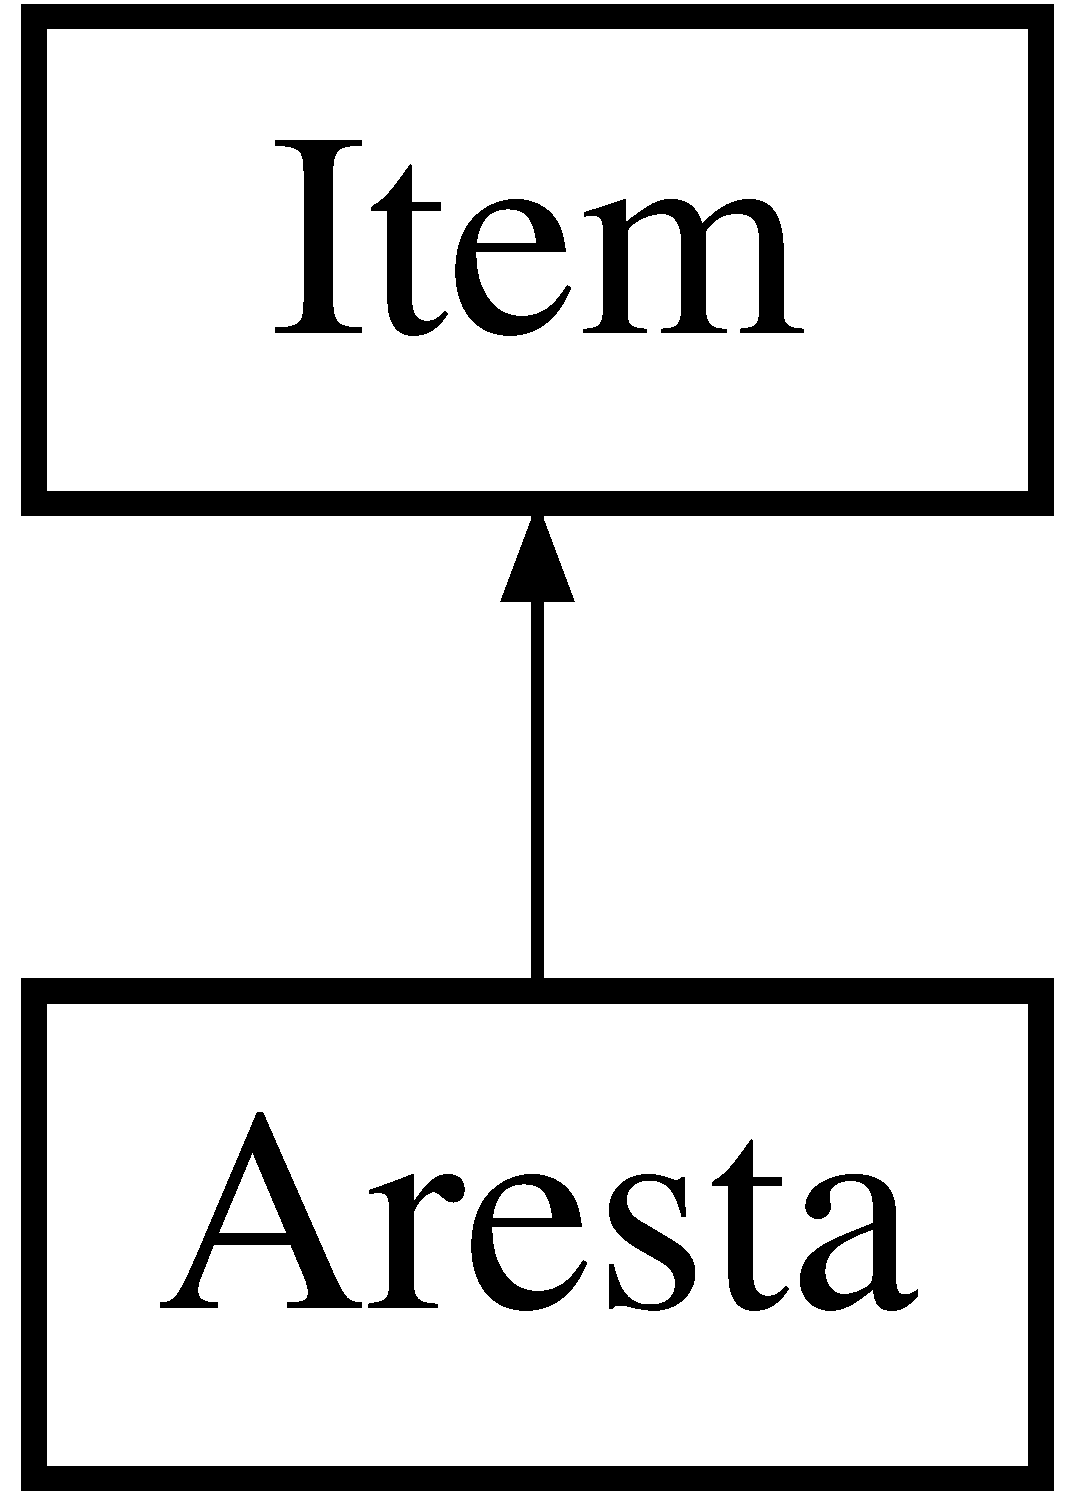
\includegraphics[height=2.000000cm]{class_aresta}
\end{center}
\end{figure}
\subsection*{Public Member Functions}
\begin{DoxyCompactItemize}
\item 
\hyperlink{class_aresta_ac4973cc1f876367f550867a6f9585710}{Aresta} (int id\-\_\-vert\-\_\-dst)
\item 
\hyperlink{class_aresta_ae98b01abb56c5edfe67ee8fb934d4e8a}{Aresta} (int id\-\_\-vert\-\_\-dst, float \hyperlink{class_aresta_a5cbe0615f1b11fc59b24743c751c7c89}{peso})
\item 
\hyperlink{class_aresta_af2ed777b341fb131f9914724a2ac034e}{Aresta} (int id\-\_\-vert\-\_\-ori, int id\-\_\-vert\-\_\-dst, float \hyperlink{class_aresta_a5cbe0615f1b11fc59b24743c751c7c89}{peso})
\item 
int \hyperlink{class_aresta_a826de2a611158755e0c3945c29d8dba7}{pega\-Id\-Destino} ()
\item 
int \hyperlink{class_aresta_ad605bd3f09038baf4623699187a31d9b}{pega\-Id\-Origem} ()
\item 
float \hyperlink{class_aresta_aabc9bf8cd3c86e3b0535b83a2495ab74}{pega\-Peso} ()
\end{DoxyCompactItemize}
\subsection*{Static Public Member Functions}
\begin{DoxyCompactItemize}
\item 
static bool \hyperlink{class_aresta_a5397827613569c129c2ba3385ce0665f}{ordena\-Aresta\-Peso} (const \hyperlink{class_aresta}{Aresta} $\ast$a1, const \hyperlink{class_aresta}{Aresta} $\ast$a2)
\end{DoxyCompactItemize}
\subsection*{Public Attributes}
\begin{DoxyCompactItemize}
\item 
float \hyperlink{class_aresta_a5cbe0615f1b11fc59b24743c751c7c89}{peso}
\end{DoxyCompactItemize}
\subsection*{Additional Inherited Members}


\subsection{Constructor \& Destructor Documentation}
\hypertarget{class_aresta_ac4973cc1f876367f550867a6f9585710}{\index{Aresta@{Aresta}!Aresta@{Aresta}}
\index{Aresta@{Aresta}!Aresta@{Aresta}}
\subsubsection[{Aresta}]{\setlength{\rightskip}{0pt plus 5cm}Aresta\-::\-Aresta (
\begin{DoxyParamCaption}
\item[{int}]{id\-\_\-vert\-\_\-dst}
\end{DoxyParamCaption}
)\hspace{0.3cm}{\ttfamily [inline]}}}\label{class_aresta_ac4973cc1f876367f550867a6f9585710}
\hypertarget{class_aresta_ae98b01abb56c5edfe67ee8fb934d4e8a}{\index{Aresta@{Aresta}!Aresta@{Aresta}}
\index{Aresta@{Aresta}!Aresta@{Aresta}}
\subsubsection[{Aresta}]{\setlength{\rightskip}{0pt plus 5cm}Aresta\-::\-Aresta (
\begin{DoxyParamCaption}
\item[{int}]{id\-\_\-vert\-\_\-dst, }
\item[{float}]{peso}
\end{DoxyParamCaption}
)\hspace{0.3cm}{\ttfamily [inline]}}}\label{class_aresta_ae98b01abb56c5edfe67ee8fb934d4e8a}
\hypertarget{class_aresta_af2ed777b341fb131f9914724a2ac034e}{\index{Aresta@{Aresta}!Aresta@{Aresta}}
\index{Aresta@{Aresta}!Aresta@{Aresta}}
\subsubsection[{Aresta}]{\setlength{\rightskip}{0pt plus 5cm}Aresta\-::\-Aresta (
\begin{DoxyParamCaption}
\item[{int}]{id\-\_\-vert\-\_\-ori, }
\item[{int}]{id\-\_\-vert\-\_\-dst, }
\item[{float}]{peso}
\end{DoxyParamCaption}
)\hspace{0.3cm}{\ttfamily [inline]}}}\label{class_aresta_af2ed777b341fb131f9914724a2ac034e}


\subsection{Member Function Documentation}
\hypertarget{class_aresta_a5397827613569c129c2ba3385ce0665f}{\index{Aresta@{Aresta}!ordena\-Aresta\-Peso@{ordena\-Aresta\-Peso}}
\index{ordena\-Aresta\-Peso@{ordena\-Aresta\-Peso}!Aresta@{Aresta}}
\subsubsection[{ordena\-Aresta\-Peso}]{\setlength{\rightskip}{0pt plus 5cm}bool Aresta\-::ordena\-Aresta\-Peso (
\begin{DoxyParamCaption}
\item[{const {\bf Aresta} $\ast$}]{a1, }
\item[{const {\bf Aresta} $\ast$}]{a2}
\end{DoxyParamCaption}
)\hspace{0.3cm}{\ttfamily [static]}}}\label{class_aresta_a5397827613569c129c2ba3385ce0665f}
\hypertarget{class_aresta_a826de2a611158755e0c3945c29d8dba7}{\index{Aresta@{Aresta}!pega\-Id\-Destino@{pega\-Id\-Destino}}
\index{pega\-Id\-Destino@{pega\-Id\-Destino}!Aresta@{Aresta}}
\subsubsection[{pega\-Id\-Destino}]{\setlength{\rightskip}{0pt plus 5cm}int Aresta\-::pega\-Id\-Destino (
\begin{DoxyParamCaption}
{}
\end{DoxyParamCaption}
)\hspace{0.3cm}{\ttfamily [inline]}}}\label{class_aresta_a826de2a611158755e0c3945c29d8dba7}
\hypertarget{class_aresta_ad605bd3f09038baf4623699187a31d9b}{\index{Aresta@{Aresta}!pega\-Id\-Origem@{pega\-Id\-Origem}}
\index{pega\-Id\-Origem@{pega\-Id\-Origem}!Aresta@{Aresta}}
\subsubsection[{pega\-Id\-Origem}]{\setlength{\rightskip}{0pt plus 5cm}int Aresta\-::pega\-Id\-Origem (
\begin{DoxyParamCaption}
{}
\end{DoxyParamCaption}
)\hspace{0.3cm}{\ttfamily [inline]}}}\label{class_aresta_ad605bd3f09038baf4623699187a31d9b}
\hypertarget{class_aresta_aabc9bf8cd3c86e3b0535b83a2495ab74}{\index{Aresta@{Aresta}!pega\-Peso@{pega\-Peso}}
\index{pega\-Peso@{pega\-Peso}!Aresta@{Aresta}}
\subsubsection[{pega\-Peso}]{\setlength{\rightskip}{0pt plus 5cm}float Aresta\-::pega\-Peso (
\begin{DoxyParamCaption}
{}
\end{DoxyParamCaption}
)\hspace{0.3cm}{\ttfamily [inline]}}}\label{class_aresta_aabc9bf8cd3c86e3b0535b83a2495ab74}


\subsection{Member Data Documentation}
\hypertarget{class_aresta_a5cbe0615f1b11fc59b24743c751c7c89}{\index{Aresta@{Aresta}!peso@{peso}}
\index{peso@{peso}!Aresta@{Aresta}}
\subsubsection[{peso}]{\setlength{\rightskip}{0pt plus 5cm}float Aresta\-::peso}}\label{class_aresta_a5cbe0615f1b11fc59b24743c751c7c89}


The documentation for this class was generated from the following files\-:\begin{DoxyCompactItemize}
\item 
\hyperlink{_grafo_8h}{Grafo.\-h}\item 
\hyperlink{_grafo_8cpp}{Grafo.\-cpp}\end{DoxyCompactItemize}

\hypertarget{class_grafo}{\section{Grafo Class Reference}
\label{class_grafo}\index{Grafo@{Grafo}}
}


{\ttfamily \#include $<$Grafo.\-h$>$}

Inheritance diagram for Grafo\-:\begin{figure}[H]
\begin{center}
\leavevmode
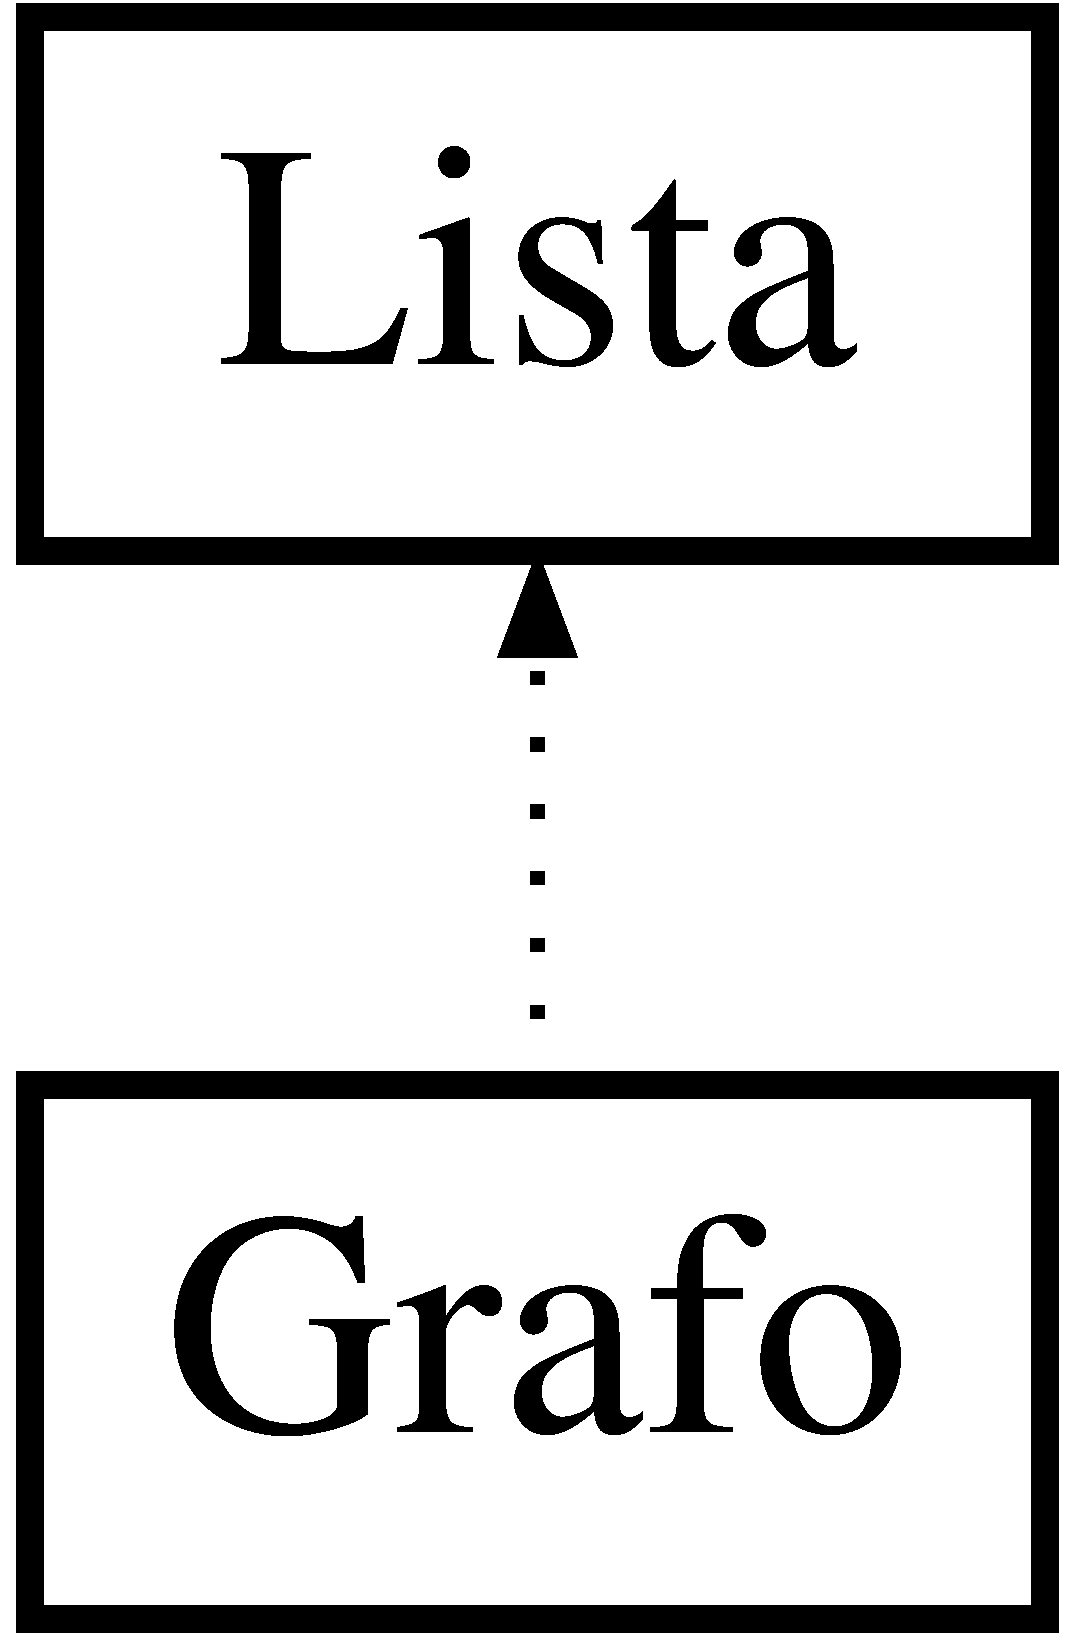
\includegraphics[height=2.000000cm]{class_grafo}
\end{center}
\end{figure}
\subsection*{Public Member Functions}
\begin{DoxyCompactItemize}
\item 
\hyperlink{class_grafo_ab810bbe26a98e9af6661ccddff66b03b}{Grafo} ()
\begin{DoxyCompactList}\small\item\em Construtor para grafo nao direcionado. \end{DoxyCompactList}\item 
\hyperlink{class_grafo_ac389a7c921f396ed4ed0f296a90a649e}{Grafo} (bool dir)
\begin{DoxyCompactList}\small\item\em Construto para grafo direcionado (digrafo). \end{DoxyCompactList}\item 
\hyperlink{class_grafo_a16f3fbba0de2667dfba3b657cb7e95ff}{$\sim$\-Grafo} ()
\begin{DoxyCompactList}\small\item\em Destrutor. \end{DoxyCompactList}\item 
void \hyperlink{class_grafo_ac422fb7b1853918b49c5b1446990ab75}{imprime\-Grafo} (\hyperlink{class_grafo}{Grafo} $\ast$g)
\begin{DoxyCompactList}\small\item\em Imprime cada vertice (no) com os nos adjacentes. \end{DoxyCompactList}\item 
void \hyperlink{class_grafo_a5eda2173b173a36459bf831cfcfd262b}{unir} (int subset\mbox{[}$\,$\mbox{]}, int v1, int v2)
\begin{DoxyCompactList}\small\item\em função para unir dois subconjuntos em um único subconjunto \end{DoxyCompactList}\item 
int \hyperlink{class_grafo_a29874190411584284934433db5bf5f99}{conta\-Nos} ()
\item 
int \hyperlink{class_grafo_a68e6656216b32cf61a2370cfcd6573a3}{retorna\-Indice} (vector$<$ int $>$ ver\-Gafo, int id)
\item 
int \hyperlink{class_grafo_a0ac5b35231457cbf54aa7d19f21b1f1e}{buscar} (int subset\mbox{[}$\,$\mbox{]}, int i)
\begin{DoxyCompactList}\small\item\em função que busca o subconjunto de um elemento \char`\"{}i\char`\"{} \end{DoxyCompactList}\item 
bool \hyperlink{class_grafo_aa5d199d9e3c9c0b7cb12fb369945e066}{eh\-A\-D\-J} (int v, int subset\mbox{[}$\,$\mbox{]})
\begin{DoxyCompactList}\small\item\em Funcoa eu verifica se o vertice v esta no subconjunto de vertice da A\-G\-M. \end{DoxyCompactList}\item 
bool \hyperlink{class_grafo_a2772417b97b45251166e8dd1e7189966}{existe\-Camonho} (\hyperlink{class_grafo}{Grafo} $\ast$g, int orin, int dest)
\item 
bool \hyperlink{class_grafo_a05bbf393596f80289b5794c98221e73a}{tana\-Lista} (int id, vector$<$ int $>$ v)
\item 
\hyperlink{class_grafo}{Grafo} $\ast$ \hyperlink{class_grafo_a4cee5922bd84c2652ad31383a61f487b}{set\-Nao\-Visitado} (\hyperlink{class_grafo}{Grafo} $\ast$g)
\begin{DoxyCompactList}\small\item\em Seta todos os vertice do \hyperlink{class_grafo}{Grafo} com nao visitao. \end{DoxyCompactList}\item 
\hyperlink{class_grafo}{Grafo} $\ast$ \hyperlink{class_grafo_a363d5b79f8ab7aaa27dea38387e9ffb6}{gera\-Grafo\-Transposto} ()
\begin{DoxyCompactList}\small\item\em Função que gera um gafos transposto invertendo das aresta de um grafo direcionado G retornando G'. \end{DoxyCompactList}\item 
vector$<$ int $>$ \hyperlink{class_grafo_a61f6a9940df187006f5c445c6d6f1aec}{ordena\-Fre\-Busca} (vector$<$ int $>$ ordem\-C, vector$<$ int $>$freq\-Nos)
\begin{DoxyCompactList}\small\item\em Ordena e frequencia resultante da busca em profundidade de forma decrescente. \end{DoxyCompactList}\item 
vector$<$ int $>$ \hyperlink{class_grafo_acd84b6964f6c1fb550a86e9d5b85fd4a}{busca\-Freq\-No\-Conexas} (\hyperlink{class_vertice}{Vertice} $\ast$v, int $\ast$cal\-Fre, vector$<$ int $>$ freq\-Nos)
\begin{DoxyCompactList}\small\item\em Retorna um vector com a ordem de cada vertice na volta da recursao de uma busca em profundidade. \end{DoxyCompactList}\item 
\hyperlink{class_vertice}{Vertice} $\ast$ \hyperlink{class_grafo_a2e8822f36da76855c6c2471731570d16}{encontra\-No} (int id)
\begin{DoxyCompactList}\small\item\em Encontra um \hyperlink{class_vertice}{Vertice} com a id e retona o vertice v se encontra. Caso nao encontre, retorna N\-U\-L\-L. \end{DoxyCompactList}\item 
\hyperlink{class_vertice}{Vertice} $\ast$ \hyperlink{class_grafo_aa6442a6688c71ad58946108cf5328213}{primeiro\-No} ()
\item 
\hyperlink{class_vertice}{Vertice} $\ast$ \hyperlink{class_grafo_ab6840a0ed069a45b57cb4140c8063d56}{proximo\-No} ()
\item 
\hyperlink{class_vertice}{Vertice} $\ast$ \hyperlink{class_grafo_a69279737c6e6f788feb2f45ffe944561}{no\-Anterior} ()
\item 
\hyperlink{class_vertice}{Vertice} $\ast$ \hyperlink{class_grafo_a4a003c3d61527160cd1e156b6f86f92e}{ultimo\-No} ()
\item 
\hyperlink{class_vertice}{Vertice} $\ast$ \hyperlink{class_grafo_a907b0bcb9e8efb64098bd799d8876399}{adiciona\-No} (int id)
\begin{DoxyCompactList}\small\item\em Adiciona um \hyperlink{class_vertice}{Vertice} com a id dada caso não exista, caso exista retorna ponteiro para o \hyperlink{class_vertice}{Vertice}. \end{DoxyCompactList}\item 
void \hyperlink{class_grafo_a9f8e73f1d74ad07d931b678adfb7066e}{adiciona\-Aresta} (int id\-\_\-origem, int id\-\_\-destino)
\begin{DoxyCompactList}\small\item\em Adiciona uma aresta em id\-\_\-origem, apontando (quando pertinente) para id\-\_\-destino. \end{DoxyCompactList}\item 
void \hyperlink{class_grafo_a6c406dd5c7eaaed2dbd1d80528b14972}{adiciona\-Aresta} (int id\-\_\-origem, int id\-\_\-destino, float peso)
\begin{DoxyCompactList}\small\item\em Adiciona uma aresta com P\-E\-S\-O, em id\-\_\-origem apontando (quando pertinente) para id\-\_\-destino. \end{DoxyCompactList}\item 
void \hyperlink{class_grafo_a1218362fe45c08e2a8d8729d5c45cbf7}{remove\-No} (int id)
\begin{DoxyCompactList}\small\item\em Procura o \hyperlink{class_vertice}{Vertice} que possui a id dada, e deleta caso encontre. \end{DoxyCompactList}\item 
void \hyperlink{class_grafo_ab3a5abe0a30afac753120ce1587f6f65}{remove\-Aresta} (int id\-\_\-no1, int id\-\_\-no2)
\begin{DoxyCompactList}\small\item\em Remove uma aresta entre dois vertices. \end{DoxyCompactList}\item 
int \hyperlink{class_grafo_a41ffeb7e79cf0d0c10297953f647c42d}{grau\-No} (int id)
\begin{DoxyCompactList}\small\item\em Retorna o grau do vertice (no) passando como parametro o id no vertice(no),. \end{DoxyCompactList}\item 
int \hyperlink{class_grafo_abada775efe72203e59e7930a095cbe95}{grau\-Grafo} ()
\begin{DoxyCompactList}\small\item\em Retorna o grau do \hyperlink{class_grafo}{Grafo}. \end{DoxyCompactList}\item 
int \hyperlink{class_grafo_ad954ce5924126084991e57a4e62a140f}{ordem\-Grafo} ()
\begin{DoxyCompactList}\small\item\em Retorna o ordem do \hyperlink{class_grafo}{Grafo}. \end{DoxyCompactList}\item 
bool \hyperlink{class_grafo_af70414fca091d884dd3d2656bdc790a9}{eh\-Trivial} ()
\begin{DoxyCompactList}\small\item\em Verifica se o grafo eh trivial. \end{DoxyCompactList}\item 
bool \hyperlink{class_grafo_a843e8d52e587e7564b4db61c8e3856e8}{eh\-Nulo} ()
\begin{DoxyCompactList}\small\item\em Verifica se o grafo eh nulo. \end{DoxyCompactList}\item 
bool \hyperlink{class_grafo_a8b8a37db83f48a3dba72ad5d68077ed7}{k\-Regular} (int id)
\begin{DoxyCompactList}\small\item\em Verifica se o grafo é K-\/\-Regular. \end{DoxyCompactList}\item 
bool \hyperlink{class_grafo_a47f39f75d015f8c35bfa71d7a3da1bfa}{completo} ()
\begin{DoxyCompactList}\small\item\em Verifica se o grafo eh completo. \end{DoxyCompactList}\item 
bool \hyperlink{class_grafo_a1fba4f1f969c2dc07171fc294506e2f6}{eh\-Multigrafo} ()
\begin{DoxyCompactList}\small\item\em Verifica se eh um Multigrafo. \end{DoxyCompactList}\item 
bool \hyperlink{class_grafo_ad7d5ff431a1cb3c909b4bbc67e52b459}{eh\-Bipartido} (\hyperlink{class_vertice}{Vertice} $\ast$v, bool muda\-Part)
\begin{DoxyCompactList}\small\item\em Verifica se eh um Bipartido. \end{DoxyCompactList}\item 
\hyperlink{class_grafo}{Grafo} $\ast$ \hyperlink{class_grafo_ab34ab3006a5efe61e3416557a855e326}{vizinhaca\-Aberta} (int id)
\begin{DoxyCompactList}\small\item\em Retorna um subgrafo induzido com os vertices adjacentes ao vertice(no) informado. \end{DoxyCompactList}\item 
\hyperlink{class_grafo}{Grafo} $\ast$ \hyperlink{class_grafo_abe28762d544d99e502c83f00ede75ddf}{vizinhaca\-Fechada} (int id)
\begin{DoxyCompactList}\small\item\em Retorna um subgrafo induzido com os vertices adjacentes ao vertice(no) informado incluindo o proprio vertice. \end{DoxyCompactList}\item 
pair$<$ \hyperlink{class_grafo}{Grafo} $\ast$, float $>$ \hyperlink{class_grafo_a9415f8df731388c329f64e8cd0c5391b}{menor\-Caminho} (int id\-\_\-origem, int id\-\_\-destino)
\begin{DoxyCompactList}\small\item\em Retorna um subgrafo com o menor caminho entre dois vertice(no) utilizando o Dijkstra. \end{DoxyCompactList}\item 
void \hyperlink{class_grafo_aa5db00b08590804c1885d383ce67d1d2}{fecho\-Transitivo\-Direto} (int id)
\begin{DoxyCompactList}\small\item\em A função gera o fecho transitivo direto dado um id de um vértice. \end{DoxyCompactList}\item 
void \hyperlink{class_grafo_a568fd7e7ef01a0bb6e85b44999f519cd}{fecho\-Transitivo\-Indireto} (int id)
\begin{DoxyCompactList}\small\item\em A função gera o fecho transitivo indireto dado um id de um vertice. \end{DoxyCompactList}\item 
bool \hyperlink{class_grafo_adf78302a0ba04265275889cecd67be01}{eh\-Multi\-Digrafo} ()
\begin{DoxyCompactList}\small\item\em Verifica se eh um Multidigrafo. \end{DoxyCompactList}\item 
bool \hyperlink{class_grafo_a50fe04d01b2d34b777d8df0b827bedab}{conexo} ()
\begin{DoxyCompactList}\small\item\em Verifica se o grafo eh conexo. \end{DoxyCompactList}\item 
bool \hyperlink{class_grafo_a184ed3a4401ad77ff33a47da71d15e24}{nos\-Sao\-Adjacentes} (int id1, int id2)
\begin{DoxyCompactList}\small\item\em Verifica se o nos sao adjacentes. \end{DoxyCompactList}\item 
bool \hyperlink{class_grafo_af095a9c01a8762f358a2c7fced700975}{mesma\-Componente\-Conexa} (int id1, int id2)
\begin{DoxyCompactList}\small\item\em Verifica se dois vertices estao em uma mesmo conponente conexa. \end{DoxyCompactList}\item 
bool \hyperlink{class_grafo_af5c44085a44be2520c52775efc87380f}{no\-Articulacao} (int id)
\begin{DoxyCompactList}\small\item\em verifica se o no eh de articulacao \end{DoxyCompactList}\item 
bool \hyperlink{class_grafo_ad5ae61b6d0ae27569dd58b519b359927}{aresta\-Ponte} (int id1, int id2)
\begin{DoxyCompactList}\small\item\em verifica se a aresta é ponte \end{DoxyCompactList}\item 
vector$<$ vector$<$ int $>$ $>$ \hyperlink{class_grafo_a42f883ece5986fcf8cbc4a8c793844f5}{quant\-Comp\-Conexo} ()
\begin{DoxyCompactList}\small\item\em Retorna a quantidade de componentes conexas do grafo em uma matrix de vector. \end{DoxyCompactList}\item 
vector$<$ vector$<$ int $>$ $>$ \hyperlink{class_grafo_ab64d335140e23a281f9600b764b6ed80}{quant\-Comp\-Forte\-Conexos} ()
\begin{DoxyCompactList}\small\item\em Funcao que retona as componentes fortemente conexas criando um array com as ordem dos vertice no retorno de uma busca em profundidade. Ao encontrar esse numeracao, e criado um grafo transposto( grafo G com as aresta invertidas). Depois e realizada uma busca em profundidade no grafo G' e as componete conexa de G' sao as componentes fortemente conexas de G. \end{DoxyCompactList}\item 
\hyperlink{class_grafo}{Grafo} $\ast$ \hyperlink{class_grafo_a8d382797529db17eaf6b77cc9c6e1de9}{Prim} (vector$<$ int $>$ ver\-Gafo)
\begin{DoxyCompactList}\small\item\em Funcao Prim para encontrar a arvore gerado minima. \end{DoxyCompactList}\item 
\hyperlink{class_grafo}{Grafo} $\ast$ \hyperlink{class_grafo_a5e15346d9279bebe36bcfe34837a194a}{Kruskal} (vector$<$ \hyperlink{class_aresta}{Aresta} $\ast$ $>$ are)
\begin{DoxyCompactList}\small\item\em Funcao kruskal que em contra um arvore geradora minima recebendo como parametro um vector comtendo as arestas ordemadas de forma crecente em relacao ao peso. \end{DoxyCompactList}\end{DoxyCompactItemize}
\subsection*{Static Public Member Functions}
\begin{DoxyCompactItemize}
\item 
static bool \hyperlink{class_grafo_a5dac1549cdbbc647b8a389df64f50746}{ordena\-Aresta} (const \hyperlink{class_aresta}{Aresta} $\ast$a1, const \hyperlink{class_aresta}{Aresta} $\ast$a2)
\end{DoxyCompactItemize}
\subsection*{Public Attributes}
\begin{DoxyCompactItemize}
\item 
int \hyperlink{class_grafo_a579e844e050120ab0cea14ca32e8735b}{quant\-Nos}
\end{DoxyCompactItemize}


\subsection{Constructor \& Destructor Documentation}
\hypertarget{class_grafo_ab810bbe26a98e9af6661ccddff66b03b}{\index{Grafo@{Grafo}!Grafo@{Grafo}}
\index{Grafo@{Grafo}!Grafo@{Grafo}}
\subsubsection[{Grafo}]{\setlength{\rightskip}{0pt plus 5cm}Grafo\-::\-Grafo (
\begin{DoxyParamCaption}
{}
\end{DoxyParamCaption}
)}}\label{class_grafo_ab810bbe26a98e9af6661ccddff66b03b}


Construtor para grafo nao direcionado. 

\hypertarget{class_grafo_ac389a7c921f396ed4ed0f296a90a649e}{\index{Grafo@{Grafo}!Grafo@{Grafo}}
\index{Grafo@{Grafo}!Grafo@{Grafo}}
\subsubsection[{Grafo}]{\setlength{\rightskip}{0pt plus 5cm}Grafo\-::\-Grafo (
\begin{DoxyParamCaption}
\item[{bool}]{dir}
\end{DoxyParamCaption}
)}}\label{class_grafo_ac389a7c921f396ed4ed0f296a90a649e}


Construto para grafo direcionado (digrafo). 


\begin{DoxyParams}{Parameters}
{\em dir} & -\/$>$ booleano que define se o grafo é direcionado. \\
\hline
\end{DoxyParams}
\hypertarget{class_grafo_a16f3fbba0de2667dfba3b657cb7e95ff}{\index{Grafo@{Grafo}!$\sim$\-Grafo@{$\sim$\-Grafo}}
\index{$\sim$\-Grafo@{$\sim$\-Grafo}!Grafo@{Grafo}}
\subsubsection[{$\sim$\-Grafo}]{\setlength{\rightskip}{0pt plus 5cm}Grafo\-::$\sim$\-Grafo (
\begin{DoxyParamCaption}
{}
\end{DoxyParamCaption}
)}}\label{class_grafo_a16f3fbba0de2667dfba3b657cb7e95ff}


Destrutor. 



\subsection{Member Function Documentation}
\hypertarget{class_grafo_a9f8e73f1d74ad07d931b678adfb7066e}{\index{Grafo@{Grafo}!adiciona\-Aresta@{adiciona\-Aresta}}
\index{adiciona\-Aresta@{adiciona\-Aresta}!Grafo@{Grafo}}
\subsubsection[{adiciona\-Aresta}]{\setlength{\rightskip}{0pt plus 5cm}void Grafo\-::adiciona\-Aresta (
\begin{DoxyParamCaption}
\item[{int}]{id\-\_\-origem, }
\item[{int}]{id\-\_\-destino}
\end{DoxyParamCaption}
)}}\label{class_grafo_a9f8e73f1d74ad07d931b678adfb7066e}


Adiciona uma aresta em id\-\_\-origem, apontando (quando pertinente) para id\-\_\-destino. 


\begin{DoxyParams}{Parameters}
{\em id\-\_\-origem} & -\/$>$ Origem da aresta. \\
\hline
{\em id\-\_\-destino} & -\/$>$ Destino da aresta. \\
\hline
\end{DoxyParams}
\hypertarget{class_grafo_a6c406dd5c7eaaed2dbd1d80528b14972}{\index{Grafo@{Grafo}!adiciona\-Aresta@{adiciona\-Aresta}}
\index{adiciona\-Aresta@{adiciona\-Aresta}!Grafo@{Grafo}}
\subsubsection[{adiciona\-Aresta}]{\setlength{\rightskip}{0pt plus 5cm}void Grafo\-::adiciona\-Aresta (
\begin{DoxyParamCaption}
\item[{int}]{id\-\_\-origem, }
\item[{int}]{id\-\_\-destino, }
\item[{float}]{peso}
\end{DoxyParamCaption}
)}}\label{class_grafo_a6c406dd5c7eaaed2dbd1d80528b14972}


Adiciona uma aresta com P\-E\-S\-O, em id\-\_\-origem apontando (quando pertinente) para id\-\_\-destino. 


\begin{DoxyParams}{Parameters}
{\em id\-\_\-origem} & -\/$>$ Origem da aresta. \\
\hline
{\em id\-\_\-destino} & -\/$>$ Destino da aresta. \\
\hline
{\em peso} & -\/$>$ Peso da aresta. \\
\hline
\end{DoxyParams}
\hypertarget{class_grafo_a907b0bcb9e8efb64098bd799d8876399}{\index{Grafo@{Grafo}!adiciona\-No@{adiciona\-No}}
\index{adiciona\-No@{adiciona\-No}!Grafo@{Grafo}}
\subsubsection[{adiciona\-No}]{\setlength{\rightskip}{0pt plus 5cm}{\bf Vertice} $\ast$ Grafo\-::adiciona\-No (
\begin{DoxyParamCaption}
\item[{int}]{id}
\end{DoxyParamCaption}
)}}\label{class_grafo_a907b0bcb9e8efb64098bd799d8876399}


Adiciona um \hyperlink{class_vertice}{Vertice} com a id dada caso não exista, caso exista retorna ponteiro para o \hyperlink{class_vertice}{Vertice}. 


\begin{DoxyParams}{Parameters}
{\em id} & -\/$>$ Identificador do vertice. \\
\hline
\end{DoxyParams}
\begin{DoxyReturn}{Returns}
v -\/$>$ Retorna um vertice. 
\end{DoxyReturn}
\hypertarget{class_grafo_ad5ae61b6d0ae27569dd58b519b359927}{\index{Grafo@{Grafo}!aresta\-Ponte@{aresta\-Ponte}}
\index{aresta\-Ponte@{aresta\-Ponte}!Grafo@{Grafo}}
\subsubsection[{aresta\-Ponte}]{\setlength{\rightskip}{0pt plus 5cm}bool Grafo\-::aresta\-Ponte (
\begin{DoxyParamCaption}
\item[{int}]{id1, }
\item[{int}]{id2}
\end{DoxyParamCaption}
)}}\label{class_grafo_ad5ae61b6d0ae27569dd58b519b359927}


verifica se a aresta é ponte 


\begin{DoxyParams}{Parameters}
{\em int} & id1 \\
\hline
{\em int} & id2 \\
\hline
\end{DoxyParams}
\begin{DoxyReturn}{Returns}
bool 
\end{DoxyReturn}
\hypertarget{class_grafo_acd84b6964f6c1fb550a86e9d5b85fd4a}{\index{Grafo@{Grafo}!busca\-Freq\-No\-Conexas@{busca\-Freq\-No\-Conexas}}
\index{busca\-Freq\-No\-Conexas@{busca\-Freq\-No\-Conexas}!Grafo@{Grafo}}
\subsubsection[{busca\-Freq\-No\-Conexas}]{\setlength{\rightskip}{0pt plus 5cm}vector$<$ int $>$ Grafo\-::busca\-Freq\-No\-Conexas (
\begin{DoxyParamCaption}
\item[{{\bf Vertice} $\ast$}]{v, }
\item[{int $\ast$}]{cal\-Fre, }
\item[{vector$<$ int $>$}]{freq\-Nos}
\end{DoxyParamCaption}
)}}\label{class_grafo_acd84b6964f6c1fb550a86e9d5b85fd4a}


Retorna um vector com a ordem de cada vertice na volta da recursao de uma busca em profundidade. 


\begin{DoxyParams}{Parameters}
{\em \hyperlink{class_vertice}{Vertice}} & $\ast$v \\
\hline
{\em int} & $\ast$cal\-Fre \\
\hline
{\em vector$<$int$>$} & freq\-Nos \\
\hline
\end{DoxyParams}
\begin{DoxyReturn}{Returns}
vector$<$int$>$ freq\-Nos 
\end{DoxyReturn}
\hypertarget{class_grafo_a0ac5b35231457cbf54aa7d19f21b1f1e}{\index{Grafo@{Grafo}!buscar@{buscar}}
\index{buscar@{buscar}!Grafo@{Grafo}}
\subsubsection[{buscar}]{\setlength{\rightskip}{0pt plus 5cm}int Grafo\-::buscar (
\begin{DoxyParamCaption}
\item[{int}]{subset\mbox{[}$\,$\mbox{]}, }
\item[{int}]{i}
\end{DoxyParamCaption}
)}}\label{class_grafo_a0ac5b35231457cbf54aa7d19f21b1f1e}


função que busca o subconjunto de um elemento \char`\"{}i\char`\"{} 


\begin{DoxyParams}{Parameters}
{\em int} & subset\mbox{[}\mbox{]} \\
\hline
{\em int} & i \\
\hline
\end{DoxyParams}
\begin{DoxyReturn}{Returns}
int i 
\end{DoxyReturn}
\hypertarget{class_grafo_a47f39f75d015f8c35bfa71d7a3da1bfa}{\index{Grafo@{Grafo}!completo@{completo}}
\index{completo@{completo}!Grafo@{Grafo}}
\subsubsection[{completo}]{\setlength{\rightskip}{0pt plus 5cm}bool Grafo\-::completo (
\begin{DoxyParamCaption}
{}
\end{DoxyParamCaption}
)}}\label{class_grafo_a47f39f75d015f8c35bfa71d7a3da1bfa}


Verifica se o grafo eh completo. 

\begin{DoxyReturn}{Returns}
True para completo e false para nao completo. 
\end{DoxyReturn}
\hypertarget{class_grafo_a50fe04d01b2d34b777d8df0b827bedab}{\index{Grafo@{Grafo}!conexo@{conexo}}
\index{conexo@{conexo}!Grafo@{Grafo}}
\subsubsection[{conexo}]{\setlength{\rightskip}{0pt plus 5cm}bool Grafo\-::conexo (
\begin{DoxyParamCaption}
{}
\end{DoxyParamCaption}
)}}\label{class_grafo_a50fe04d01b2d34b777d8df0b827bedab}


Verifica se o grafo eh conexo. 

\begin{DoxyReturn}{Returns}
bool 
\end{DoxyReturn}
quantidade de vertice no grafo

quantidade de vertice visitados \hypertarget{class_grafo_a29874190411584284934433db5bf5f99}{\index{Grafo@{Grafo}!conta\-Nos@{conta\-Nos}}
\index{conta\-Nos@{conta\-Nos}!Grafo@{Grafo}}
\subsubsection[{conta\-Nos}]{\setlength{\rightskip}{0pt plus 5cm}int Grafo\-::conta\-Nos (
\begin{DoxyParamCaption}
{}
\end{DoxyParamCaption}
)\hspace{0.3cm}{\ttfamily [inline]}}}\label{class_grafo_a29874190411584284934433db5bf5f99}
\hypertarget{class_grafo_aa5d199d9e3c9c0b7cb12fb369945e066}{\index{Grafo@{Grafo}!eh\-A\-D\-J@{eh\-A\-D\-J}}
\index{eh\-A\-D\-J@{eh\-A\-D\-J}!Grafo@{Grafo}}
\subsubsection[{eh\-A\-D\-J}]{\setlength{\rightskip}{0pt plus 5cm}bool Grafo\-::eh\-A\-D\-J (
\begin{DoxyParamCaption}
\item[{int}]{v, }
\item[{int}]{subset\mbox{[}$\,$\mbox{]}}
\end{DoxyParamCaption}
)}}\label{class_grafo_aa5d199d9e3c9c0b7cb12fb369945e066}


Funcoa eu verifica se o vertice v esta no subconjunto de vertice da A\-G\-M. 


\begin{DoxyParams}{Parameters}
{\em int} & v -\/$>$ vertice v \\
\hline
{\em int} & subset\mbox{[}\mbox{]} -\/$>$ subconjunto de vertice da A\-G\-M \\
\hline
\end{DoxyParams}
\begin{DoxyReturn}{Returns}
bool 
\end{DoxyReturn}
\hypertarget{class_grafo_ad7d5ff431a1cb3c909b4bbc67e52b459}{\index{Grafo@{Grafo}!eh\-Bipartido@{eh\-Bipartido}}
\index{eh\-Bipartido@{eh\-Bipartido}!Grafo@{Grafo}}
\subsubsection[{eh\-Bipartido}]{\setlength{\rightskip}{0pt plus 5cm}bool Grafo\-::eh\-Bipartido (
\begin{DoxyParamCaption}
\item[{{\bf Vertice} $\ast$}]{v, }
\item[{bool}]{muda\-Part}
\end{DoxyParamCaption}
)}}\label{class_grafo_ad7d5ff431a1cb3c909b4bbc67e52b459}


Verifica se eh um Bipartido. 


\begin{DoxyParams}{Parameters}
{\em v} & -\/$>$ primeiro vertice da lista. \\
\hline
{\em muda\-Part} & -\/$>$ Booleano que altera a partcao do vertice. \\
\hline
\end{DoxyParams}
\begin{DoxyReturn}{Returns}
True para bipartido e false para nao bipartido. 
\end{DoxyReturn}
\hypertarget{class_grafo_adf78302a0ba04265275889cecd67be01}{\index{Grafo@{Grafo}!eh\-Multi\-Digrafo@{eh\-Multi\-Digrafo}}
\index{eh\-Multi\-Digrafo@{eh\-Multi\-Digrafo}!Grafo@{Grafo}}
\subsubsection[{eh\-Multi\-Digrafo}]{\setlength{\rightskip}{0pt plus 5cm}bool Grafo\-::eh\-Multi\-Digrafo (
\begin{DoxyParamCaption}
{}
\end{DoxyParamCaption}
)}}\label{class_grafo_adf78302a0ba04265275889cecd67be01}


Verifica se eh um Multidigrafo. 

\begin{DoxyReturn}{Returns}
True para Multi\-Digrafo e false para nao Multi\-Digrafo. 
\end{DoxyReturn}
\hypertarget{class_grafo_a1fba4f1f969c2dc07171fc294506e2f6}{\index{Grafo@{Grafo}!eh\-Multigrafo@{eh\-Multigrafo}}
\index{eh\-Multigrafo@{eh\-Multigrafo}!Grafo@{Grafo}}
\subsubsection[{eh\-Multigrafo}]{\setlength{\rightskip}{0pt plus 5cm}bool Grafo\-::eh\-Multigrafo (
\begin{DoxyParamCaption}
{}
\end{DoxyParamCaption}
)}}\label{class_grafo_a1fba4f1f969c2dc07171fc294506e2f6}


Verifica se eh um Multigrafo. 

\begin{DoxyReturn}{Returns}
True para Multigrafo e false para nao Multigrafo. 
\end{DoxyReturn}
\hypertarget{class_grafo_a843e8d52e587e7564b4db61c8e3856e8}{\index{Grafo@{Grafo}!eh\-Nulo@{eh\-Nulo}}
\index{eh\-Nulo@{eh\-Nulo}!Grafo@{Grafo}}
\subsubsection[{eh\-Nulo}]{\setlength{\rightskip}{0pt plus 5cm}bool Grafo\-::eh\-Nulo (
\begin{DoxyParamCaption}
{}
\end{DoxyParamCaption}
)}}\label{class_grafo_a843e8d52e587e7564b4db61c8e3856e8}


Verifica se o grafo eh nulo. 

\begin{DoxyReturn}{Returns}
True para nulo e false para nao nulo. 
\end{DoxyReturn}
\hypertarget{class_grafo_af70414fca091d884dd3d2656bdc790a9}{\index{Grafo@{Grafo}!eh\-Trivial@{eh\-Trivial}}
\index{eh\-Trivial@{eh\-Trivial}!Grafo@{Grafo}}
\subsubsection[{eh\-Trivial}]{\setlength{\rightskip}{0pt plus 5cm}bool Grafo\-::eh\-Trivial (
\begin{DoxyParamCaption}
{}
\end{DoxyParamCaption}
)}}\label{class_grafo_af70414fca091d884dd3d2656bdc790a9}


Verifica se o grafo eh trivial. 

\begin{DoxyReturn}{Returns}
True para trivial e false para nao trivial. 
\end{DoxyReturn}
\hypertarget{class_grafo_a2e8822f36da76855c6c2471731570d16}{\index{Grafo@{Grafo}!encontra\-No@{encontra\-No}}
\index{encontra\-No@{encontra\-No}!Grafo@{Grafo}}
\subsubsection[{encontra\-No}]{\setlength{\rightskip}{0pt plus 5cm}{\bf Vertice} $\ast$ Grafo\-::encontra\-No (
\begin{DoxyParamCaption}
\item[{int}]{id}
\end{DoxyParamCaption}
)}}\label{class_grafo_a2e8822f36da76855c6c2471731570d16}


Encontra um \hyperlink{class_vertice}{Vertice} com a id e retona o vertice v se encontra. Caso nao encontre, retorna N\-U\-L\-L. 


\begin{DoxyParams}{Parameters}
{\em int} & id \\
\hline
\end{DoxyParams}
\begin{DoxyReturn}{Returns}
\hyperlink{class_vertice}{Vertice} $\ast$v 
\end{DoxyReturn}
\hypertarget{class_grafo_a2772417b97b45251166e8dd1e7189966}{\index{Grafo@{Grafo}!existe\-Camonho@{existe\-Camonho}}
\index{existe\-Camonho@{existe\-Camonho}!Grafo@{Grafo}}
\subsubsection[{existe\-Camonho}]{\setlength{\rightskip}{0pt plus 5cm}bool Grafo\-::existe\-Camonho (
\begin{DoxyParamCaption}
\item[{{\bf Grafo} $\ast$}]{g, }
\item[{int}]{orin, }
\item[{int}]{dest}
\end{DoxyParamCaption}
)}}\label{class_grafo_a2772417b97b45251166e8dd1e7189966}
\hypertarget{class_grafo_aa5db00b08590804c1885d383ce67d1d2}{\index{Grafo@{Grafo}!fecho\-Transitivo\-Direto@{fecho\-Transitivo\-Direto}}
\index{fecho\-Transitivo\-Direto@{fecho\-Transitivo\-Direto}!Grafo@{Grafo}}
\subsubsection[{fecho\-Transitivo\-Direto}]{\setlength{\rightskip}{0pt plus 5cm}void Grafo\-::fecho\-Transitivo\-Direto (
\begin{DoxyParamCaption}
\item[{int}]{id}
\end{DoxyParamCaption}
)}}\label{class_grafo_aa5db00b08590804c1885d383ce67d1d2}


A função gera o fecho transitivo direto dado um id de um vértice. 


\begin{DoxyParams}{Parameters}
{\em int} & id \\
\hline
\end{DoxyParams}
\hypertarget{class_grafo_a568fd7e7ef01a0bb6e85b44999f519cd}{\index{Grafo@{Grafo}!fecho\-Transitivo\-Indireto@{fecho\-Transitivo\-Indireto}}
\index{fecho\-Transitivo\-Indireto@{fecho\-Transitivo\-Indireto}!Grafo@{Grafo}}
\subsubsection[{fecho\-Transitivo\-Indireto}]{\setlength{\rightskip}{0pt plus 5cm}void Grafo\-::fecho\-Transitivo\-Indireto (
\begin{DoxyParamCaption}
\item[{int}]{id}
\end{DoxyParamCaption}
)}}\label{class_grafo_a568fd7e7ef01a0bb6e85b44999f519cd}


A função gera o fecho transitivo indireto dado um id de um vertice. 


\begin{DoxyParams}{Parameters}
{\em int} & id \\
\hline
\end{DoxyParams}
\hypertarget{class_grafo_a363d5b79f8ab7aaa27dea38387e9ffb6}{\index{Grafo@{Grafo}!gera\-Grafo\-Transposto@{gera\-Grafo\-Transposto}}
\index{gera\-Grafo\-Transposto@{gera\-Grafo\-Transposto}!Grafo@{Grafo}}
\subsubsection[{gera\-Grafo\-Transposto}]{\setlength{\rightskip}{0pt plus 5cm}{\bf Grafo} $\ast$ Grafo\-::gera\-Grafo\-Transposto (
\begin{DoxyParamCaption}
{}
\end{DoxyParamCaption}
)}}\label{class_grafo_a363d5b79f8ab7aaa27dea38387e9ffb6}


Função que gera um gafos transposto invertendo das aresta de um grafo direcionado G retornando G'. 

\begin{DoxyReturn}{Returns}
Grafo$\ast$ gt 
\end{DoxyReturn}
\hypertarget{class_grafo_abada775efe72203e59e7930a095cbe95}{\index{Grafo@{Grafo}!grau\-Grafo@{grau\-Grafo}}
\index{grau\-Grafo@{grau\-Grafo}!Grafo@{Grafo}}
\subsubsection[{grau\-Grafo}]{\setlength{\rightskip}{0pt plus 5cm}int Grafo\-::grau\-Grafo (
\begin{DoxyParamCaption}
{}
\end{DoxyParamCaption}
)}}\label{class_grafo_abada775efe72203e59e7930a095cbe95}


Retorna o grau do \hyperlink{class_grafo}{Grafo}. 

\begin{DoxyReturn}{Returns}
maior -\/$>$ Grau do grafo . 
\end{DoxyReturn}
\hypertarget{class_grafo_a41ffeb7e79cf0d0c10297953f647c42d}{\index{Grafo@{Grafo}!grau\-No@{grau\-No}}
\index{grau\-No@{grau\-No}!Grafo@{Grafo}}
\subsubsection[{grau\-No}]{\setlength{\rightskip}{0pt plus 5cm}int Grafo\-::grau\-No (
\begin{DoxyParamCaption}
\item[{int}]{id}
\end{DoxyParamCaption}
)}}\label{class_grafo_a41ffeb7e79cf0d0c10297953f647c42d}


Retorna o grau do vertice (no) passando como parametro o id no vertice(no),. 


\begin{DoxyParams}{Parameters}
{\em id} & -\/$>$ Identificador do vertice. \\
\hline
\end{DoxyParams}
\begin{DoxyReturn}{Returns}
grau -\/$>$ Grau do no. 
\end{DoxyReturn}
\hypertarget{class_grafo_ac422fb7b1853918b49c5b1446990ab75}{\index{Grafo@{Grafo}!imprime\-Grafo@{imprime\-Grafo}}
\index{imprime\-Grafo@{imprime\-Grafo}!Grafo@{Grafo}}
\subsubsection[{imprime\-Grafo}]{\setlength{\rightskip}{0pt plus 5cm}void Grafo\-::imprime\-Grafo (
\begin{DoxyParamCaption}
\item[{{\bf Grafo} $\ast$}]{g}
\end{DoxyParamCaption}
)}}\label{class_grafo_ac422fb7b1853918b49c5b1446990ab75}


Imprime cada vertice (no) com os nos adjacentes. 


\begin{DoxyParams}{Parameters}
{\em Grafo$\ast$} & g \\
\hline
\end{DoxyParams}
\hypertarget{class_grafo_a8b8a37db83f48a3dba72ad5d68077ed7}{\index{Grafo@{Grafo}!k\-Regular@{k\-Regular}}
\index{k\-Regular@{k\-Regular}!Grafo@{Grafo}}
\subsubsection[{k\-Regular}]{\setlength{\rightskip}{0pt plus 5cm}bool Grafo\-::k\-Regular (
\begin{DoxyParamCaption}
\item[{int}]{id}
\end{DoxyParamCaption}
)}}\label{class_grafo_a8b8a37db83f48a3dba72ad5d68077ed7}


Verifica se o grafo é K-\/\-Regular. 

\begin{DoxyReturn}{Returns}
True para k-\/regular e false para nao k-\/regular. 
\end{DoxyReturn}
\hypertarget{class_grafo_a5e15346d9279bebe36bcfe34837a194a}{\index{Grafo@{Grafo}!Kruskal@{Kruskal}}
\index{Kruskal@{Kruskal}!Grafo@{Grafo}}
\subsubsection[{Kruskal}]{\setlength{\rightskip}{0pt plus 5cm}{\bf Grafo} $\ast$ Grafo\-::\-Kruskal (
\begin{DoxyParamCaption}
\item[{vector$<$ {\bf Aresta} $\ast$ $>$}]{are}
\end{DoxyParamCaption}
)}}\label{class_grafo_a5e15346d9279bebe36bcfe34837a194a}


Funcao kruskal que em contra um arvore geradora minima recebendo como parametro um vector comtendo as arestas ordemadas de forma crecente em relacao ao peso. 


\begin{DoxyParams}{Parameters}
{\em vector$<$\-Aresta$\ast$$>$} & are \\
\hline
\end{DoxyParams}
\begin{DoxyReturn}{Returns}
Grafo$\ast$ ar; 
\end{DoxyReturn}
\hypertarget{class_grafo_a9415f8df731388c329f64e8cd0c5391b}{\index{Grafo@{Grafo}!menor\-Caminho@{menor\-Caminho}}
\index{menor\-Caminho@{menor\-Caminho}!Grafo@{Grafo}}
\subsubsection[{menor\-Caminho}]{\setlength{\rightskip}{0pt plus 5cm}pair$<$ {\bf Grafo} $\ast$, float $>$ Grafo\-::menor\-Caminho (
\begin{DoxyParamCaption}
\item[{int}]{id\-\_\-origem, }
\item[{int}]{id\-\_\-destino}
\end{DoxyParamCaption}
)}}\label{class_grafo_a9415f8df731388c329f64e8cd0c5391b}


Retorna um subgrafo com o menor caminho entre dois vertice(no) utilizando o Dijkstra. 

\begin{DoxyReturn}{Returns}
\hyperlink{class_grafo}{Grafo} 
\end{DoxyReturn}
\hypertarget{class_grafo_af095a9c01a8762f358a2c7fced700975}{\index{Grafo@{Grafo}!mesma\-Componente\-Conexa@{mesma\-Componente\-Conexa}}
\index{mesma\-Componente\-Conexa@{mesma\-Componente\-Conexa}!Grafo@{Grafo}}
\subsubsection[{mesma\-Componente\-Conexa}]{\setlength{\rightskip}{0pt plus 5cm}bool Grafo\-::mesma\-Componente\-Conexa (
\begin{DoxyParamCaption}
\item[{int}]{id1, }
\item[{int}]{id2}
\end{DoxyParamCaption}
)}}\label{class_grafo_af095a9c01a8762f358a2c7fced700975}


Verifica se dois vertices estao em uma mesmo conponente conexa. 


\begin{DoxyParams}{Parameters}
{\em int} & id1 \\
\hline
{\em int} & id2 \\
\hline
\end{DoxyParams}
\begin{DoxyReturn}{Returns}
bool 
\end{DoxyReturn}
\hypertarget{class_grafo_a69279737c6e6f788feb2f45ffe944561}{\index{Grafo@{Grafo}!no\-Anterior@{no\-Anterior}}
\index{no\-Anterior@{no\-Anterior}!Grafo@{Grafo}}
\subsubsection[{no\-Anterior}]{\setlength{\rightskip}{0pt plus 5cm}{\bf Vertice}$\ast$ Grafo\-::no\-Anterior (
\begin{DoxyParamCaption}
{}
\end{DoxyParamCaption}
)\hspace{0.3cm}{\ttfamily [inline]}}}\label{class_grafo_a69279737c6e6f788feb2f45ffe944561}
\hypertarget{class_grafo_af5c44085a44be2520c52775efc87380f}{\index{Grafo@{Grafo}!no\-Articulacao@{no\-Articulacao}}
\index{no\-Articulacao@{no\-Articulacao}!Grafo@{Grafo}}
\subsubsection[{no\-Articulacao}]{\setlength{\rightskip}{0pt plus 5cm}bool Grafo\-::no\-Articulacao (
\begin{DoxyParamCaption}
\item[{int}]{id}
\end{DoxyParamCaption}
)}}\label{class_grafo_af5c44085a44be2520c52775efc87380f}


verifica se o no eh de articulacao 


\begin{DoxyParams}{Parameters}
{\em int} & id \\
\hline
\end{DoxyParams}
\begin{DoxyReturn}{Returns}
bool 
\end{DoxyReturn}
\hypertarget{class_grafo_a184ed3a4401ad77ff33a47da71d15e24}{\index{Grafo@{Grafo}!nos\-Sao\-Adjacentes@{nos\-Sao\-Adjacentes}}
\index{nos\-Sao\-Adjacentes@{nos\-Sao\-Adjacentes}!Grafo@{Grafo}}
\subsubsection[{nos\-Sao\-Adjacentes}]{\setlength{\rightskip}{0pt plus 5cm}bool Grafo\-::nos\-Sao\-Adjacentes (
\begin{DoxyParamCaption}
\item[{int}]{id1, }
\item[{int}]{id2}
\end{DoxyParamCaption}
)}}\label{class_grafo_a184ed3a4401ad77ff33a47da71d15e24}


Verifica se o nos sao adjacentes. 


\begin{DoxyParams}{Parameters}
{\em int} & id1 \\
\hline
{\em int} & id2 \\
\hline
\end{DoxyParams}
\begin{DoxyReturn}{Returns}
bool 
\end{DoxyReturn}
\hypertarget{class_grafo_ad954ce5924126084991e57a4e62a140f}{\index{Grafo@{Grafo}!ordem\-Grafo@{ordem\-Grafo}}
\index{ordem\-Grafo@{ordem\-Grafo}!Grafo@{Grafo}}
\subsubsection[{ordem\-Grafo}]{\setlength{\rightskip}{0pt plus 5cm}int Grafo\-::ordem\-Grafo (
\begin{DoxyParamCaption}
{}
\end{DoxyParamCaption}
)}}\label{class_grafo_ad954ce5924126084991e57a4e62a140f}


Retorna o ordem do \hyperlink{class_grafo}{Grafo}. 

\begin{DoxyReturn}{Returns}
inteiro que repesenta a ordem do grafo. 
\end{DoxyReturn}
\hypertarget{class_grafo_a5dac1549cdbbc647b8a389df64f50746}{\index{Grafo@{Grafo}!ordena\-Aresta@{ordena\-Aresta}}
\index{ordena\-Aresta@{ordena\-Aresta}!Grafo@{Grafo}}
\subsubsection[{ordena\-Aresta}]{\setlength{\rightskip}{0pt plus 5cm}static bool Grafo\-::ordena\-Aresta (
\begin{DoxyParamCaption}
\item[{const {\bf Aresta} $\ast$}]{a1, }
\item[{const {\bf Aresta} $\ast$}]{a2}
\end{DoxyParamCaption}
)\hspace{0.3cm}{\ttfamily [static]}}}\label{class_grafo_a5dac1549cdbbc647b8a389df64f50746}
\hypertarget{class_grafo_a61f6a9940df187006f5c445c6d6f1aec}{\index{Grafo@{Grafo}!ordena\-Fre\-Busca@{ordena\-Fre\-Busca}}
\index{ordena\-Fre\-Busca@{ordena\-Fre\-Busca}!Grafo@{Grafo}}
\subsubsection[{ordena\-Fre\-Busca}]{\setlength{\rightskip}{0pt plus 5cm}vector$<$ int $>$ Grafo\-::ordena\-Fre\-Busca (
\begin{DoxyParamCaption}
\item[{vector$<$ int $>$}]{ordem\-C, }
\item[{vector$<$ int $>$}]{freq\-Nos}
\end{DoxyParamCaption}
)}}\label{class_grafo_a61f6a9940df187006f5c445c6d6f1aec}


Ordena e frequencia resultante da busca em profundidade de forma decrescente. 


\begin{DoxyParams}{Parameters}
{\em int} & freq\-Nos\mbox{[}\mbox{]} \\
\hline
\end{DoxyParams}
\begin{DoxyReturn}{Returns}
vector$<$int$>$ ordem\-C 
\end{DoxyReturn}
\hypertarget{class_grafo_a8d382797529db17eaf6b77cc9c6e1de9}{\index{Grafo@{Grafo}!Prim@{Prim}}
\index{Prim@{Prim}!Grafo@{Grafo}}
\subsubsection[{Prim}]{\setlength{\rightskip}{0pt plus 5cm}{\bf Grafo} $\ast$ Grafo\-::\-Prim (
\begin{DoxyParamCaption}
\item[{vector$<$ int $>$}]{ver\-Gafo}
\end{DoxyParamCaption}
)}}\label{class_grafo_a8d382797529db17eaf6b77cc9c6e1de9}


Funcao Prim para encontrar a arvore gerado minima. 

\begin{DoxyReturn}{Returns}
Grafo$\ast$ g 
\end{DoxyReturn}
\hypertarget{class_grafo_aa6442a6688c71ad58946108cf5328213}{\index{Grafo@{Grafo}!primeiro\-No@{primeiro\-No}}
\index{primeiro\-No@{primeiro\-No}!Grafo@{Grafo}}
\subsubsection[{primeiro\-No}]{\setlength{\rightskip}{0pt plus 5cm}{\bf Vertice}$\ast$ Grafo\-::primeiro\-No (
\begin{DoxyParamCaption}
{}
\end{DoxyParamCaption}
)\hspace{0.3cm}{\ttfamily [inline]}}}\label{class_grafo_aa6442a6688c71ad58946108cf5328213}
\hypertarget{class_grafo_ab6840a0ed069a45b57cb4140c8063d56}{\index{Grafo@{Grafo}!proximo\-No@{proximo\-No}}
\index{proximo\-No@{proximo\-No}!Grafo@{Grafo}}
\subsubsection[{proximo\-No}]{\setlength{\rightskip}{0pt plus 5cm}{\bf Vertice}$\ast$ Grafo\-::proximo\-No (
\begin{DoxyParamCaption}
{}
\end{DoxyParamCaption}
)\hspace{0.3cm}{\ttfamily [inline]}}}\label{class_grafo_ab6840a0ed069a45b57cb4140c8063d56}
\hypertarget{class_grafo_a42f883ece5986fcf8cbc4a8c793844f5}{\index{Grafo@{Grafo}!quant\-Comp\-Conexo@{quant\-Comp\-Conexo}}
\index{quant\-Comp\-Conexo@{quant\-Comp\-Conexo}!Grafo@{Grafo}}
\subsubsection[{quant\-Comp\-Conexo}]{\setlength{\rightskip}{0pt plus 5cm}vector$<$ vector$<$ int $>$ $>$ Grafo\-::quant\-Comp\-Conexo (
\begin{DoxyParamCaption}
{}
\end{DoxyParamCaption}
)}}\label{class_grafo_a42f883ece5986fcf8cbc4a8c793844f5}


Retorna a quantidade de componentes conexas do grafo em uma matrix de vector. 

\begin{DoxyReturn}{Returns}
vector $<$ vector$<$int$>$ $>$ 
\end{DoxyReturn}
\hypertarget{class_grafo_ab64d335140e23a281f9600b764b6ed80}{\index{Grafo@{Grafo}!quant\-Comp\-Forte\-Conexos@{quant\-Comp\-Forte\-Conexos}}
\index{quant\-Comp\-Forte\-Conexos@{quant\-Comp\-Forte\-Conexos}!Grafo@{Grafo}}
\subsubsection[{quant\-Comp\-Forte\-Conexos}]{\setlength{\rightskip}{0pt plus 5cm}vector$<$ vector$<$ int $>$ $>$ Grafo\-::quant\-Comp\-Forte\-Conexos (
\begin{DoxyParamCaption}
{}
\end{DoxyParamCaption}
)}}\label{class_grafo_ab64d335140e23a281f9600b764b6ed80}


Funcao que retona as componentes fortemente conexas criando um array com as ordem dos vertice no retorno de uma busca em profundidade. Ao encontrar esse numeracao, e criado um grafo transposto( grafo G com as aresta invertidas). Depois e realizada uma busca em profundidade no grafo G' e as componete conexa de G' sao as componentes fortemente conexas de G. 

\begin{DoxyReturn}{Returns}
vector$<$ vector$<$int$>$ $>$ quant\-Forte\-Conexo 
\end{DoxyReturn}
\hypertarget{class_grafo_ab3a5abe0a30afac753120ce1587f6f65}{\index{Grafo@{Grafo}!remove\-Aresta@{remove\-Aresta}}
\index{remove\-Aresta@{remove\-Aresta}!Grafo@{Grafo}}
\subsubsection[{remove\-Aresta}]{\setlength{\rightskip}{0pt plus 5cm}void Grafo\-::remove\-Aresta (
\begin{DoxyParamCaption}
\item[{int}]{id\-\_\-no1, }
\item[{int}]{id\-\_\-no2}
\end{DoxyParamCaption}
)}}\label{class_grafo_ab3a5abe0a30afac753120ce1587f6f65}


Remove uma aresta entre dois vertices. 


\begin{DoxyParams}{Parameters}
{\em id\-\_\-no1} & -\/$>$ \hyperlink{class_vertice}{Vertice} origem. \\
\hline
{\em id\-\_\-no2} & -\/$>$ \hyperlink{class_vertice}{Vertice} destino. \\
\hline
\end{DoxyParams}
\hypertarget{class_grafo_a1218362fe45c08e2a8d8729d5c45cbf7}{\index{Grafo@{Grafo}!remove\-No@{remove\-No}}
\index{remove\-No@{remove\-No}!Grafo@{Grafo}}
\subsubsection[{remove\-No}]{\setlength{\rightskip}{0pt plus 5cm}void Grafo\-::remove\-No (
\begin{DoxyParamCaption}
\item[{int}]{id}
\end{DoxyParamCaption}
)}}\label{class_grafo_a1218362fe45c08e2a8d8729d5c45cbf7}


Procura o \hyperlink{class_vertice}{Vertice} que possui a id dada, e deleta caso encontre. 


\begin{DoxyParams}{Parameters}
{\em id} & -\/$>$ Identificador do vertice. \\
\hline
\end{DoxyParams}
\hypertarget{class_grafo_a68e6656216b32cf61a2370cfcd6573a3}{\index{Grafo@{Grafo}!retorna\-Indice@{retorna\-Indice}}
\index{retorna\-Indice@{retorna\-Indice}!Grafo@{Grafo}}
\subsubsection[{retorna\-Indice}]{\setlength{\rightskip}{0pt plus 5cm}int Grafo\-::retorna\-Indice (
\begin{DoxyParamCaption}
\item[{vector$<$ int $>$}]{ver\-Gafo, }
\item[{int}]{id}
\end{DoxyParamCaption}
)}}\label{class_grafo_a68e6656216b32cf61a2370cfcd6573a3}
\hypertarget{class_grafo_a4cee5922bd84c2652ad31383a61f487b}{\index{Grafo@{Grafo}!set\-Nao\-Visitado@{set\-Nao\-Visitado}}
\index{set\-Nao\-Visitado@{set\-Nao\-Visitado}!Grafo@{Grafo}}
\subsubsection[{set\-Nao\-Visitado}]{\setlength{\rightskip}{0pt plus 5cm}{\bf Grafo} $\ast$ Grafo\-::set\-Nao\-Visitado (
\begin{DoxyParamCaption}
\item[{{\bf Grafo} $\ast$}]{g}
\end{DoxyParamCaption}
)}}\label{class_grafo_a4cee5922bd84c2652ad31383a61f487b}


Seta todos os vertice do \hyperlink{class_grafo}{Grafo} com nao visitao. 


\begin{DoxyParams}{Parameters}
{\em \hyperlink{class_grafo}{Grafo}} & $\ast$g \\
\hline
\end{DoxyParams}
\begin{DoxyReturn}{Returns}
\hyperlink{class_grafo}{Grafo} $\ast$g 
\end{DoxyReturn}
\hypertarget{class_grafo_a05bbf393596f80289b5794c98221e73a}{\index{Grafo@{Grafo}!tana\-Lista@{tana\-Lista}}
\index{tana\-Lista@{tana\-Lista}!Grafo@{Grafo}}
\subsubsection[{tana\-Lista}]{\setlength{\rightskip}{0pt plus 5cm}bool Grafo\-::tana\-Lista (
\begin{DoxyParamCaption}
\item[{int}]{id, }
\item[{vector$<$ int $>$}]{v}
\end{DoxyParamCaption}
)}}\label{class_grafo_a05bbf393596f80289b5794c98221e73a}
\hypertarget{class_grafo_a4a003c3d61527160cd1e156b6f86f92e}{\index{Grafo@{Grafo}!ultimo\-No@{ultimo\-No}}
\index{ultimo\-No@{ultimo\-No}!Grafo@{Grafo}}
\subsubsection[{ultimo\-No}]{\setlength{\rightskip}{0pt plus 5cm}{\bf Vertice}$\ast$ Grafo\-::ultimo\-No (
\begin{DoxyParamCaption}
{}
\end{DoxyParamCaption}
)\hspace{0.3cm}{\ttfamily [inline]}}}\label{class_grafo_a4a003c3d61527160cd1e156b6f86f92e}
\hypertarget{class_grafo_a5eda2173b173a36459bf831cfcfd262b}{\index{Grafo@{Grafo}!unir@{unir}}
\index{unir@{unir}!Grafo@{Grafo}}
\subsubsection[{unir}]{\setlength{\rightskip}{0pt plus 5cm}void Grafo\-::unir (
\begin{DoxyParamCaption}
\item[{int}]{subset\mbox{[}$\,$\mbox{]}, }
\item[{int}]{v1, }
\item[{int}]{v2}
\end{DoxyParamCaption}
)}}\label{class_grafo_a5eda2173b173a36459bf831cfcfd262b}


função para unir dois subconjuntos em um único subconjunto 


\begin{DoxyParams}{Parameters}
{\em int} & subset\mbox{[}\mbox{]} subconjunto resuntante \\
\hline
{\em int} & v1 subconjunto 1 \\
\hline
{\em int} & v2 subconjunto 2 \\
\hline
\end{DoxyParams}
\begin{DoxyReturn}{Returns}

\end{DoxyReturn}
\hypertarget{class_grafo_ab34ab3006a5efe61e3416557a855e326}{\index{Grafo@{Grafo}!vizinhaca\-Aberta@{vizinhaca\-Aberta}}
\index{vizinhaca\-Aberta@{vizinhaca\-Aberta}!Grafo@{Grafo}}
\subsubsection[{vizinhaca\-Aberta}]{\setlength{\rightskip}{0pt plus 5cm}{\bf Grafo} $\ast$ Grafo\-::vizinhaca\-Aberta (
\begin{DoxyParamCaption}
\item[{int}]{id}
\end{DoxyParamCaption}
)}}\label{class_grafo_ab34ab3006a5efe61e3416557a855e326}


Retorna um subgrafo induzido com os vertices adjacentes ao vertice(no) informado. 


\begin{DoxyParams}{Parameters}
{\em int} & id \\
\hline
\end{DoxyParams}
\begin{DoxyReturn}{Returns}
\hyperlink{class_grafo}{Grafo} 
\end{DoxyReturn}
\hypertarget{class_grafo_abe28762d544d99e502c83f00ede75ddf}{\index{Grafo@{Grafo}!vizinhaca\-Fechada@{vizinhaca\-Fechada}}
\index{vizinhaca\-Fechada@{vizinhaca\-Fechada}!Grafo@{Grafo}}
\subsubsection[{vizinhaca\-Fechada}]{\setlength{\rightskip}{0pt plus 5cm}{\bf Grafo} $\ast$ Grafo\-::vizinhaca\-Fechada (
\begin{DoxyParamCaption}
\item[{int}]{id}
\end{DoxyParamCaption}
)}}\label{class_grafo_abe28762d544d99e502c83f00ede75ddf}


Retorna um subgrafo induzido com os vertices adjacentes ao vertice(no) informado incluindo o proprio vertice. 


\begin{DoxyParams}{Parameters}
{\em int} & id \\
\hline
\end{DoxyParams}
\begin{DoxyReturn}{Returns}
\hyperlink{class_grafo}{Grafo} 
\end{DoxyReturn}


\subsection{Member Data Documentation}
\hypertarget{class_grafo_a579e844e050120ab0cea14ca32e8735b}{\index{Grafo@{Grafo}!quant\-Nos@{quant\-Nos}}
\index{quant\-Nos@{quant\-Nos}!Grafo@{Grafo}}
\subsubsection[{quant\-Nos}]{\setlength{\rightskip}{0pt plus 5cm}int Grafo\-::quant\-Nos}}\label{class_grafo_a579e844e050120ab0cea14ca32e8735b}


The documentation for this class was generated from the following files\-:\begin{DoxyCompactItemize}
\item 
\hyperlink{_grafo_8h}{Grafo.\-h}\item 
\hyperlink{_grafo_8cpp}{Grafo.\-cpp}\end{DoxyCompactItemize}

\hypertarget{class_item}{\section{Item Class Reference}
\label{class_item}\index{Item@{Item}}
}


{\ttfamily \#include $<$Lista.\-h$>$}

Inheritance diagram for Item\-:\begin{figure}[H]
\begin{center}
\leavevmode
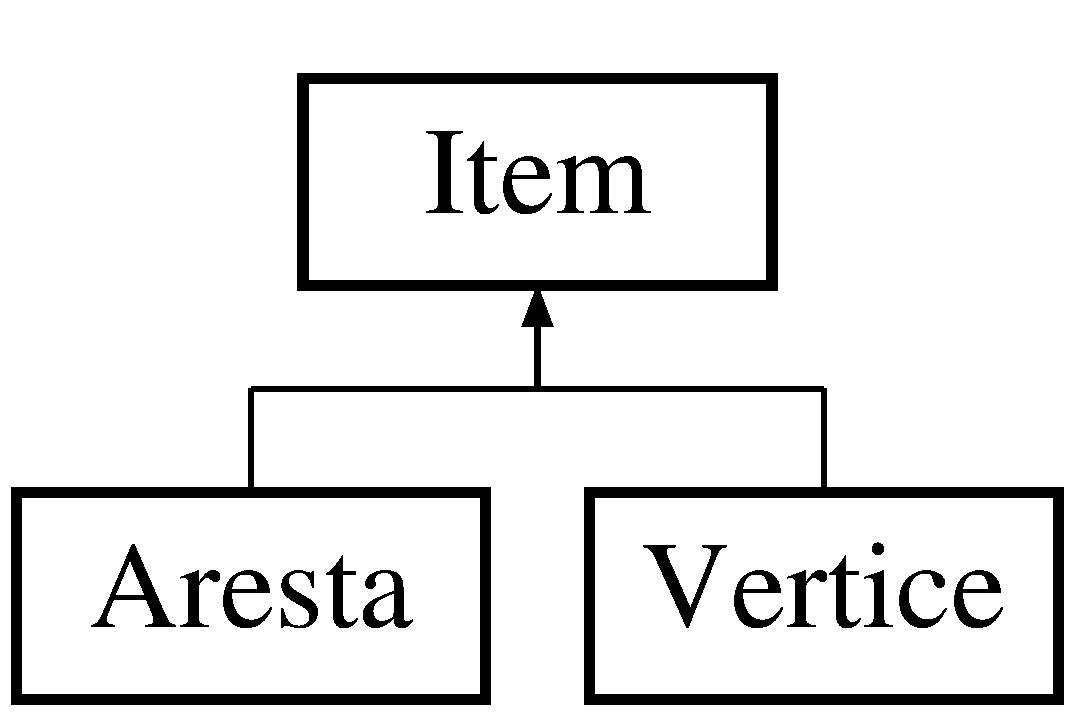
\includegraphics[height=2.000000cm]{class_item}
\end{center}
\end{figure}
\subsection*{Public Member Functions}
\begin{DoxyCompactItemize}
\item 
\hyperlink{class_item_a297720c02984eab37332ae795d22189d}{Item} ()
\item 
void \hyperlink{class_item_aeea06d242803e4fedbbe98cc36f5b6d9}{seta\-Prox} (\hyperlink{class_item}{Item} $\ast$\hyperlink{class_item_aa80cddac5a6f4213726fbf01045cf604}{prox})
\item 
void \hyperlink{class_item_a7e8bf0cd525f073018792deb778cf5d2}{seta\-Ant} (\hyperlink{class_item}{Item} $\ast$\hyperlink{class_item_aac7756495b3c31f38745064f17088dd1}{ant})
\item 
void \hyperlink{class_item_a162ade7dabf9bc6f3bd7909cde0620cc}{seta\-Info} (int \hyperlink{class_item_aa9042dad3a101d42bb82c9073dc01915}{info})
\item 
\hyperlink{class_item}{Item} $\ast$ \hyperlink{class_item_a06100877bf190da9ebdbe4ef9fec7718}{pega\-Prox} ()
\item 
\hyperlink{class_item}{Item} $\ast$ \hyperlink{class_item_a07a1d22091bc2e65e5db0482e3797dae}{pega\-Ant} ()
\item 
int \hyperlink{class_item_a42ae965c0740df01e65af042364f1582}{pega\-Info} ()
\end{DoxyCompactItemize}
\subsection*{Protected Attributes}
\begin{DoxyCompactItemize}
\item 
\hyperlink{class_item}{Item} $\ast$ \hyperlink{class_item_aac7756495b3c31f38745064f17088dd1}{ant}
\begin{DoxyCompactList}\small\item\em \hyperlink{class_item}{Item} anterior. \end{DoxyCompactList}\item 
\hyperlink{class_item}{Item} $\ast$ \hyperlink{class_item_aa80cddac5a6f4213726fbf01045cf604}{prox}
\begin{DoxyCompactList}\small\item\em Proximo item. \end{DoxyCompactList}\item 
int \hyperlink{class_item_aa9042dad3a101d42bb82c9073dc01915}{info}
\begin{DoxyCompactList}\small\item\em Representecao do vertice. \end{DoxyCompactList}\end{DoxyCompactItemize}


\subsection{Constructor \& Destructor Documentation}
\hypertarget{class_item_a297720c02984eab37332ae795d22189d}{\index{Item@{Item}!Item@{Item}}
\index{Item@{Item}!Item@{Item}}
\subsubsection[{Item}]{\setlength{\rightskip}{0pt plus 5cm}Item\-::\-Item (
\begin{DoxyParamCaption}
{}
\end{DoxyParamCaption}
)\hspace{0.3cm}{\ttfamily [inline]}}}\label{class_item_a297720c02984eab37332ae795d22189d}


\subsection{Member Function Documentation}
\hypertarget{class_item_a07a1d22091bc2e65e5db0482e3797dae}{\index{Item@{Item}!pega\-Ant@{pega\-Ant}}
\index{pega\-Ant@{pega\-Ant}!Item@{Item}}
\subsubsection[{pega\-Ant}]{\setlength{\rightskip}{0pt plus 5cm}{\bf Item}$\ast$ Item\-::pega\-Ant (
\begin{DoxyParamCaption}
{}
\end{DoxyParamCaption}
)\hspace{0.3cm}{\ttfamily [inline]}}}\label{class_item_a07a1d22091bc2e65e5db0482e3797dae}
\hypertarget{class_item_a42ae965c0740df01e65af042364f1582}{\index{Item@{Item}!pega\-Info@{pega\-Info}}
\index{pega\-Info@{pega\-Info}!Item@{Item}}
\subsubsection[{pega\-Info}]{\setlength{\rightskip}{0pt plus 5cm}int Item\-::pega\-Info (
\begin{DoxyParamCaption}
{}
\end{DoxyParamCaption}
)\hspace{0.3cm}{\ttfamily [inline]}}}\label{class_item_a42ae965c0740df01e65af042364f1582}
\hypertarget{class_item_a06100877bf190da9ebdbe4ef9fec7718}{\index{Item@{Item}!pega\-Prox@{pega\-Prox}}
\index{pega\-Prox@{pega\-Prox}!Item@{Item}}
\subsubsection[{pega\-Prox}]{\setlength{\rightskip}{0pt plus 5cm}{\bf Item}$\ast$ Item\-::pega\-Prox (
\begin{DoxyParamCaption}
{}
\end{DoxyParamCaption}
)\hspace{0.3cm}{\ttfamily [inline]}}}\label{class_item_a06100877bf190da9ebdbe4ef9fec7718}
\hypertarget{class_item_a7e8bf0cd525f073018792deb778cf5d2}{\index{Item@{Item}!seta\-Ant@{seta\-Ant}}
\index{seta\-Ant@{seta\-Ant}!Item@{Item}}
\subsubsection[{seta\-Ant}]{\setlength{\rightskip}{0pt plus 5cm}void Item\-::seta\-Ant (
\begin{DoxyParamCaption}
\item[{{\bf Item} $\ast$}]{ant}
\end{DoxyParamCaption}
)\hspace{0.3cm}{\ttfamily [inline]}}}\label{class_item_a7e8bf0cd525f073018792deb778cf5d2}
\hypertarget{class_item_a162ade7dabf9bc6f3bd7909cde0620cc}{\index{Item@{Item}!seta\-Info@{seta\-Info}}
\index{seta\-Info@{seta\-Info}!Item@{Item}}
\subsubsection[{seta\-Info}]{\setlength{\rightskip}{0pt plus 5cm}void Item\-::seta\-Info (
\begin{DoxyParamCaption}
\item[{int}]{info}
\end{DoxyParamCaption}
)\hspace{0.3cm}{\ttfamily [inline]}}}\label{class_item_a162ade7dabf9bc6f3bd7909cde0620cc}
\hypertarget{class_item_aeea06d242803e4fedbbe98cc36f5b6d9}{\index{Item@{Item}!seta\-Prox@{seta\-Prox}}
\index{seta\-Prox@{seta\-Prox}!Item@{Item}}
\subsubsection[{seta\-Prox}]{\setlength{\rightskip}{0pt plus 5cm}void Item\-::seta\-Prox (
\begin{DoxyParamCaption}
\item[{{\bf Item} $\ast$}]{prox}
\end{DoxyParamCaption}
)\hspace{0.3cm}{\ttfamily [inline]}}}\label{class_item_aeea06d242803e4fedbbe98cc36f5b6d9}


\subsection{Member Data Documentation}
\hypertarget{class_item_aac7756495b3c31f38745064f17088dd1}{\index{Item@{Item}!ant@{ant}}
\index{ant@{ant}!Item@{Item}}
\subsubsection[{ant}]{\setlength{\rightskip}{0pt plus 5cm}{\bf Item}$\ast$ Item\-::ant\hspace{0.3cm}{\ttfamily [protected]}}}\label{class_item_aac7756495b3c31f38745064f17088dd1}


\hyperlink{class_item}{Item} anterior. 

\hypertarget{class_item_aa9042dad3a101d42bb82c9073dc01915}{\index{Item@{Item}!info@{info}}
\index{info@{info}!Item@{Item}}
\subsubsection[{info}]{\setlength{\rightskip}{0pt plus 5cm}int Item\-::info\hspace{0.3cm}{\ttfamily [protected]}}}\label{class_item_aa9042dad3a101d42bb82c9073dc01915}


Representecao do vertice. 

\hypertarget{class_item_aa80cddac5a6f4213726fbf01045cf604}{\index{Item@{Item}!prox@{prox}}
\index{prox@{prox}!Item@{Item}}
\subsubsection[{prox}]{\setlength{\rightskip}{0pt plus 5cm}{\bf Item}$\ast$ Item\-::prox\hspace{0.3cm}{\ttfamily [protected]}}}\label{class_item_aa80cddac5a6f4213726fbf01045cf604}


Proximo item. 



The documentation for this class was generated from the following file\-:\begin{DoxyCompactItemize}
\item 
\hyperlink{_lista_8h}{Lista.\-h}\end{DoxyCompactItemize}

\hypertarget{class_leitura_gravacao}{\section{Leitura\-Gravacao Class Reference}
\label{class_leitura_gravacao}\index{Leitura\-Gravacao@{Leitura\-Gravacao}}
}


{\ttfamily \#include $<$Leitura\-Gravacao.\-h$>$}

\subsection*{Public Member Functions}
\begin{DoxyCompactItemize}
\item 
\hyperlink{class_grafo}{Grafo} $\ast$ \hyperlink{class_leitura_gravacao_ae8d26b77bde160493638bc5ab63e08ab}{ler\-Arquivo} (char $\ast$ar, \hyperlink{class_grafo}{Grafo} $\ast$gd)
\begin{DoxyCompactList}\small\item\em Funçao que le e adiciona o vertice em um grafo G. \end{DoxyCompactList}\item 
void \hyperlink{class_leitura_gravacao_a48039a206ba69bd10ee8ac517e586ac9}{grava\-Arquivo} (char $\ast$nom\-Arquivo, vector$<$ vector$<$ int $>$ $>$com\-Forte\-Conexo)
\begin{DoxyCompactList}\small\item\em Funcao que gera um arquivo com as componetes fortemente conexa do grafo passando o nome do arquivo e um vector com as componentes. \end{DoxyCompactList}\item 
void \hyperlink{class_leitura_gravacao_a0285f216b47406414526bd9ddba4aa4f}{grava\-Arquivo} (\hyperlink{class_grafo}{Grafo} $\ast$g, char $\ast$nom\-Arquivo, int n\-Vertice, int n\-Aresta, float grau\-Medio)
\begin{DoxyCompactList}\small\item\em Funcao que gera um aquirvo com as informacoes do grafo G como frequencia de cada vertice, quantos vertice, quantas arestas e o grau medio de cada vertice. \end{DoxyCompactList}\end{DoxyCompactItemize}


\subsection{Member Function Documentation}
\hypertarget{class_leitura_gravacao_a48039a206ba69bd10ee8ac517e586ac9}{\index{Leitura\-Gravacao@{Leitura\-Gravacao}!grava\-Arquivo@{grava\-Arquivo}}
\index{grava\-Arquivo@{grava\-Arquivo}!LeituraGravacao@{Leitura\-Gravacao}}
\subsubsection[{grava\-Arquivo}]{\setlength{\rightskip}{0pt plus 5cm}void Leitura\-Gravacao\-::grava\-Arquivo (
\begin{DoxyParamCaption}
\item[{char $\ast$}]{nom\-Arquivo, }
\item[{vector$<$ vector$<$ int $>$ $>$}]{com\-Forte\-Conexo}
\end{DoxyParamCaption}
)}}\label{class_leitura_gravacao_a48039a206ba69bd10ee8ac517e586ac9}


Funcao que gera um arquivo com as componetes fortemente conexa do grafo passando o nome do arquivo e um vector com as componentes. 


\begin{DoxyParams}{Parameters}
{\em char$\ast$} & nom\-Arquivo \\
\hline
{\em vector$<$} & vector$<$int$>$ $>$ com\-Forte\-Conexo \\
\hline
\end{DoxyParams}
\hypertarget{class_leitura_gravacao_a0285f216b47406414526bd9ddba4aa4f}{\index{Leitura\-Gravacao@{Leitura\-Gravacao}!grava\-Arquivo@{grava\-Arquivo}}
\index{grava\-Arquivo@{grava\-Arquivo}!LeituraGravacao@{Leitura\-Gravacao}}
\subsubsection[{grava\-Arquivo}]{\setlength{\rightskip}{0pt plus 5cm}void Leitura\-Gravacao\-::grava\-Arquivo (
\begin{DoxyParamCaption}
\item[{{\bf Grafo} $\ast$}]{g, }
\item[{char $\ast$}]{nom\-Arquivo, }
\item[{int}]{n\-Vertice, }
\item[{int}]{n\-Aresta, }
\item[{float}]{grau\-Medio}
\end{DoxyParamCaption}
)}}\label{class_leitura_gravacao_a0285f216b47406414526bd9ddba4aa4f}


Funcao que gera um aquirvo com as informacoes do grafo G como frequencia de cada vertice, quantos vertice, quantas arestas e o grau medio de cada vertice. 


\begin{DoxyParams}{Parameters}
{\em \hyperlink{class_grafo}{Grafo}} & $\ast$g \\
\hline
{\em char$\ast$} & nom\-Arquivo \\
\hline
{\em int} & n\-Vertice \\
\hline
{\em int} & n\-Aresta \\
\hline
{\em float} & grau\-Medio \\
\hline
\end{DoxyParams}
\hypertarget{class_leitura_gravacao_ae8d26b77bde160493638bc5ab63e08ab}{\index{Leitura\-Gravacao@{Leitura\-Gravacao}!ler\-Arquivo@{ler\-Arquivo}}
\index{ler\-Arquivo@{ler\-Arquivo}!LeituraGravacao@{Leitura\-Gravacao}}
\subsubsection[{ler\-Arquivo}]{\setlength{\rightskip}{0pt plus 5cm}{\bf Grafo} $\ast$ Leitura\-Gravacao\-::ler\-Arquivo (
\begin{DoxyParamCaption}
\item[{char $\ast$}]{ar, }
\item[{{\bf Grafo} $\ast$}]{gd}
\end{DoxyParamCaption}
)}}\label{class_leitura_gravacao_ae8d26b77bde160493638bc5ab63e08ab}


Funçao que le e adiciona o vertice em um grafo G. 


\begin{DoxyParams}{Parameters}
{\em char} & $\ast$ar -\/$>$ nome do arquivo para a leitura \\
\hline
{\em \hyperlink{class_grafo}{Grafo}} & $\ast$gd -\/$>$ grafo a ser adicionados os vertices \\
\hline
\end{DoxyParams}
\begin{DoxyReturn}{Returns}
\hyperlink{class_grafo}{Grafo} $\ast$gd 
\end{DoxyReturn}


The documentation for this class was generated from the following files\-:\begin{DoxyCompactItemize}
\item 
\hyperlink{_leitura_gravacao_8h}{Leitura\-Gravacao.\-h}\item 
\hyperlink{_leitura_gravacao_8cpp}{Leitura\-Gravacao.\-cpp}\end{DoxyCompactItemize}

\hypertarget{class_lista}{\section{Lista Class Reference}
\label{class_lista}\index{Lista@{Lista}}
}


{\ttfamily \#include $<$Lista.\-h$>$}

Inheritance diagram for Lista\-:\begin{figure}[H]
\begin{center}
\leavevmode
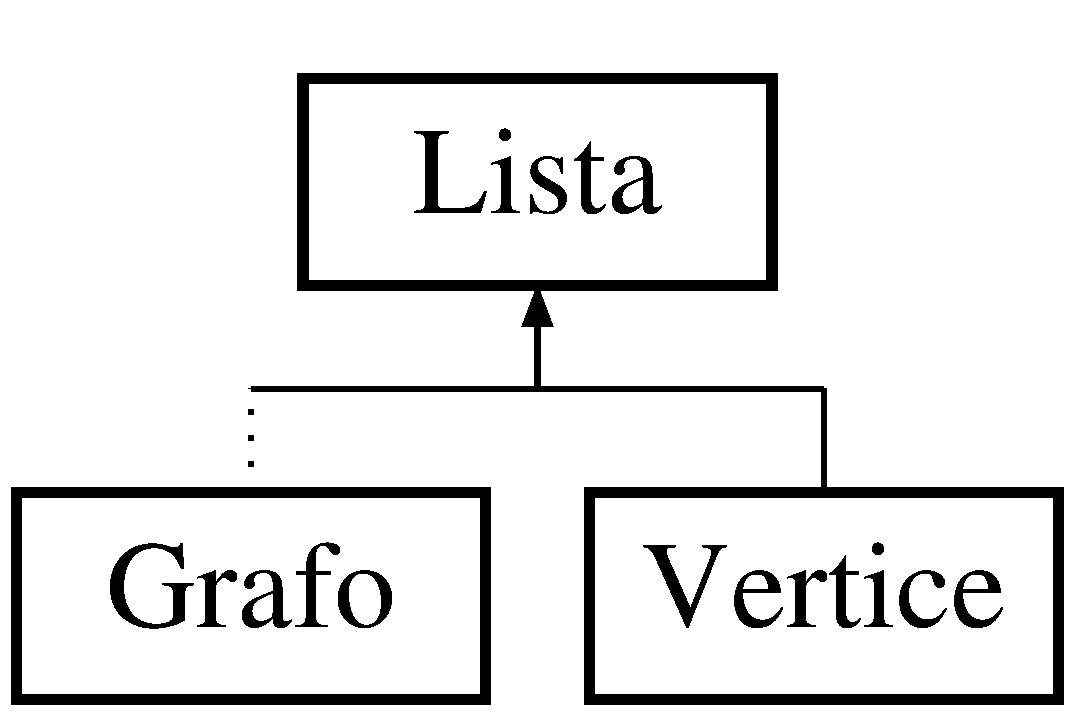
\includegraphics[height=2.000000cm]{class_lista}
\end{center}
\end{figure}
\subsection*{Public Member Functions}
\begin{DoxyCompactItemize}
\item 
\hyperlink{class_lista_a1f668b36909182ef1360b48503529a31}{Lista} ()
\item 
void \hyperlink{class_lista_a0b1e9b3728bd4b9c6ef2d9c095dbb4f4}{adiciona\-Item} (\hyperlink{class_item}{Item} $\ast$n)
\item 
void \hyperlink{class_lista_a32622b53bc0720338439beecd0e7972f}{deleta\-Item} (\hyperlink{class_item}{Item} $\ast$n)
\item 
\hyperlink{class_item}{Item} $\ast$ \hyperlink{class_lista_a21093c5b211072af96f8fda2e5739773}{inicio\-Lista} ()
\item 
\hyperlink{class_item}{Item} $\ast$ \hyperlink{class_lista_a92efd69dea7b9b4caffcf9ebf12825ef}{fim\-Lista} ()
\item 
\hyperlink{class_item}{Item} $\ast$ \hyperlink{class_lista_afd444ac095ae137b6b43e5e575e54864}{no\-Iterator} ()
\item 
\hyperlink{class_item}{Item} $\ast$ \hyperlink{class_lista_acc446a0d931b922cbdf4a61794afe658}{caminha\-Lista} ()
\item 
\hyperlink{class_item}{Item} $\ast$ \hyperlink{class_lista_aabb1d795e42a01bb8c4d3271a922ed09}{retorna\-Lista} ()
\item 
int \hyperlink{class_lista_ae006b01ac1cb5d6aba47acdc410db3f0}{conta\-Items} ()
\end{DoxyCompactItemize}
\subsection*{Protected Attributes}
\begin{DoxyCompactItemize}
\item 
\hyperlink{class_item}{Item} $\ast$ \hyperlink{class_lista_a7c35eadb33738c21dad896e957eff430}{pri}
\begin{DoxyCompactList}\small\item\em Primeiro elemento da lista. \end{DoxyCompactList}\item 
\hyperlink{class_item}{Item} $\ast$ \hyperlink{class_lista_a89bce7d87b5cd06297851d19d9be4a10}{ult}
\begin{DoxyCompactList}\small\item\em Ultimo elemento da lista. \end{DoxyCompactList}\item 
\hyperlink{class_item}{Item} $\ast$ \hyperlink{class_lista_a2e5f3aba3731dfddf41016ade510d3aa}{it}
\begin{DoxyCompactList}\small\item\em Interador. \end{DoxyCompactList}\item 
int \hyperlink{class_lista_a6d17539dfc71dde4df05343fcfefb8b0}{nitems}
\begin{DoxyCompactList}\small\item\em Numeros de Itens. \end{DoxyCompactList}\end{DoxyCompactItemize}


\subsection{Constructor \& Destructor Documentation}
\hypertarget{class_lista_a1f668b36909182ef1360b48503529a31}{\index{Lista@{Lista}!Lista@{Lista}}
\index{Lista@{Lista}!Lista@{Lista}}
\subsubsection[{Lista}]{\setlength{\rightskip}{0pt plus 5cm}Lista\-::\-Lista (
\begin{DoxyParamCaption}
{}
\end{DoxyParamCaption}
)\hspace{0.3cm}{\ttfamily [inline]}}}\label{class_lista_a1f668b36909182ef1360b48503529a31}


\subsection{Member Function Documentation}
\hypertarget{class_lista_a0b1e9b3728bd4b9c6ef2d9c095dbb4f4}{\index{Lista@{Lista}!adiciona\-Item@{adiciona\-Item}}
\index{adiciona\-Item@{adiciona\-Item}!Lista@{Lista}}
\subsubsection[{adiciona\-Item}]{\setlength{\rightskip}{0pt plus 5cm}void Lista\-::adiciona\-Item (
\begin{DoxyParamCaption}
\item[{{\bf Item} $\ast$}]{n}
\end{DoxyParamCaption}
)}}\label{class_lista_a0b1e9b3728bd4b9c6ef2d9c095dbb4f4}
Primeiro item

Segundo item

Qualquer outro item

Contador de items \hypertarget{class_lista_acc446a0d931b922cbdf4a61794afe658}{\index{Lista@{Lista}!caminha\-Lista@{caminha\-Lista}}
\index{caminha\-Lista@{caminha\-Lista}!Lista@{Lista}}
\subsubsection[{caminha\-Lista}]{\setlength{\rightskip}{0pt plus 5cm}{\bf Item}$\ast$ Lista\-::caminha\-Lista (
\begin{DoxyParamCaption}
{}
\end{DoxyParamCaption}
)\hspace{0.3cm}{\ttfamily [inline]}}}\label{class_lista_acc446a0d931b922cbdf4a61794afe658}
\hypertarget{class_lista_ae006b01ac1cb5d6aba47acdc410db3f0}{\index{Lista@{Lista}!conta\-Items@{conta\-Items}}
\index{conta\-Items@{conta\-Items}!Lista@{Lista}}
\subsubsection[{conta\-Items}]{\setlength{\rightskip}{0pt plus 5cm}int Lista\-::conta\-Items (
\begin{DoxyParamCaption}
{}
\end{DoxyParamCaption}
)\hspace{0.3cm}{\ttfamily [inline]}}}\label{class_lista_ae006b01ac1cb5d6aba47acdc410db3f0}
\hypertarget{class_lista_a32622b53bc0720338439beecd0e7972f}{\index{Lista@{Lista}!deleta\-Item@{deleta\-Item}}
\index{deleta\-Item@{deleta\-Item}!Lista@{Lista}}
\subsubsection[{deleta\-Item}]{\setlength{\rightskip}{0pt plus 5cm}void Lista\-::deleta\-Item (
\begin{DoxyParamCaption}
\item[{{\bf Item} $\ast$}]{n}
\end{DoxyParamCaption}
)}}\label{class_lista_a32622b53bc0720338439beecd0e7972f}
Condições de saída imediata

Tem apenas 1 elemento

Tem apenas 2 elementos

É o primeiro da lista

É o ultimo da lista

Para qualquer outra quantidade de elementos

Anterior a N

Sucessor de N

Relocar o iterator caso estejamos deletando o ponteiro para o qual ele aponta

Contador de items \hypertarget{class_lista_a92efd69dea7b9b4caffcf9ebf12825ef}{\index{Lista@{Lista}!fim\-Lista@{fim\-Lista}}
\index{fim\-Lista@{fim\-Lista}!Lista@{Lista}}
\subsubsection[{fim\-Lista}]{\setlength{\rightskip}{0pt plus 5cm}{\bf Item}$\ast$ Lista\-::fim\-Lista (
\begin{DoxyParamCaption}
{}
\end{DoxyParamCaption}
)\hspace{0.3cm}{\ttfamily [inline]}}}\label{class_lista_a92efd69dea7b9b4caffcf9ebf12825ef}
\hypertarget{class_lista_a21093c5b211072af96f8fda2e5739773}{\index{Lista@{Lista}!inicio\-Lista@{inicio\-Lista}}
\index{inicio\-Lista@{inicio\-Lista}!Lista@{Lista}}
\subsubsection[{inicio\-Lista}]{\setlength{\rightskip}{0pt plus 5cm}{\bf Item}$\ast$ Lista\-::inicio\-Lista (
\begin{DoxyParamCaption}
{}
\end{DoxyParamCaption}
)\hspace{0.3cm}{\ttfamily [inline]}}}\label{class_lista_a21093c5b211072af96f8fda2e5739773}
\hypertarget{class_lista_afd444ac095ae137b6b43e5e575e54864}{\index{Lista@{Lista}!no\-Iterator@{no\-Iterator}}
\index{no\-Iterator@{no\-Iterator}!Lista@{Lista}}
\subsubsection[{no\-Iterator}]{\setlength{\rightskip}{0pt plus 5cm}{\bf Item}$\ast$ Lista\-::no\-Iterator (
\begin{DoxyParamCaption}
{}
\end{DoxyParamCaption}
)\hspace{0.3cm}{\ttfamily [inline]}}}\label{class_lista_afd444ac095ae137b6b43e5e575e54864}
\hypertarget{class_lista_aabb1d795e42a01bb8c4d3271a922ed09}{\index{Lista@{Lista}!retorna\-Lista@{retorna\-Lista}}
\index{retorna\-Lista@{retorna\-Lista}!Lista@{Lista}}
\subsubsection[{retorna\-Lista}]{\setlength{\rightskip}{0pt plus 5cm}{\bf Item}$\ast$ Lista\-::retorna\-Lista (
\begin{DoxyParamCaption}
{}
\end{DoxyParamCaption}
)\hspace{0.3cm}{\ttfamily [inline]}}}\label{class_lista_aabb1d795e42a01bb8c4d3271a922ed09}


\subsection{Member Data Documentation}
\hypertarget{class_lista_a2e5f3aba3731dfddf41016ade510d3aa}{\index{Lista@{Lista}!it@{it}}
\index{it@{it}!Lista@{Lista}}
\subsubsection[{it}]{\setlength{\rightskip}{0pt plus 5cm}{\bf Item}$\ast$ Lista\-::it\hspace{0.3cm}{\ttfamily [protected]}}}\label{class_lista_a2e5f3aba3731dfddf41016ade510d3aa}


Interador. 

\hypertarget{class_lista_a6d17539dfc71dde4df05343fcfefb8b0}{\index{Lista@{Lista}!nitems@{nitems}}
\index{nitems@{nitems}!Lista@{Lista}}
\subsubsection[{nitems}]{\setlength{\rightskip}{0pt plus 5cm}int Lista\-::nitems\hspace{0.3cm}{\ttfamily [protected]}}}\label{class_lista_a6d17539dfc71dde4df05343fcfefb8b0}


Numeros de Itens. 

\hypertarget{class_lista_a7c35eadb33738c21dad896e957eff430}{\index{Lista@{Lista}!pri@{pri}}
\index{pri@{pri}!Lista@{Lista}}
\subsubsection[{pri}]{\setlength{\rightskip}{0pt plus 5cm}{\bf Item}$\ast$ Lista\-::pri\hspace{0.3cm}{\ttfamily [protected]}}}\label{class_lista_a7c35eadb33738c21dad896e957eff430}


Primeiro elemento da lista. 

\hypertarget{class_lista_a89bce7d87b5cd06297851d19d9be4a10}{\index{Lista@{Lista}!ult@{ult}}
\index{ult@{ult}!Lista@{Lista}}
\subsubsection[{ult}]{\setlength{\rightskip}{0pt plus 5cm}{\bf Item}$\ast$ Lista\-::ult\hspace{0.3cm}{\ttfamily [protected]}}}\label{class_lista_a89bce7d87b5cd06297851d19d9be4a10}


Ultimo elemento da lista. 



The documentation for this class was generated from the following files\-:\begin{DoxyCompactItemize}
\item 
\hyperlink{_lista_8h}{Lista.\-h}\item 
\hyperlink{_lista_8cpp}{Lista.\-cpp}\end{DoxyCompactItemize}

\hypertarget{class_vertice}{\section{Vertice Class Reference}
\label{class_vertice}\index{Vertice@{Vertice}}
}


{\ttfamily \#include $<$Grafo.\-h$>$}

Inheritance diagram for Vertice\-:\begin{figure}[H]
\begin{center}
\leavevmode
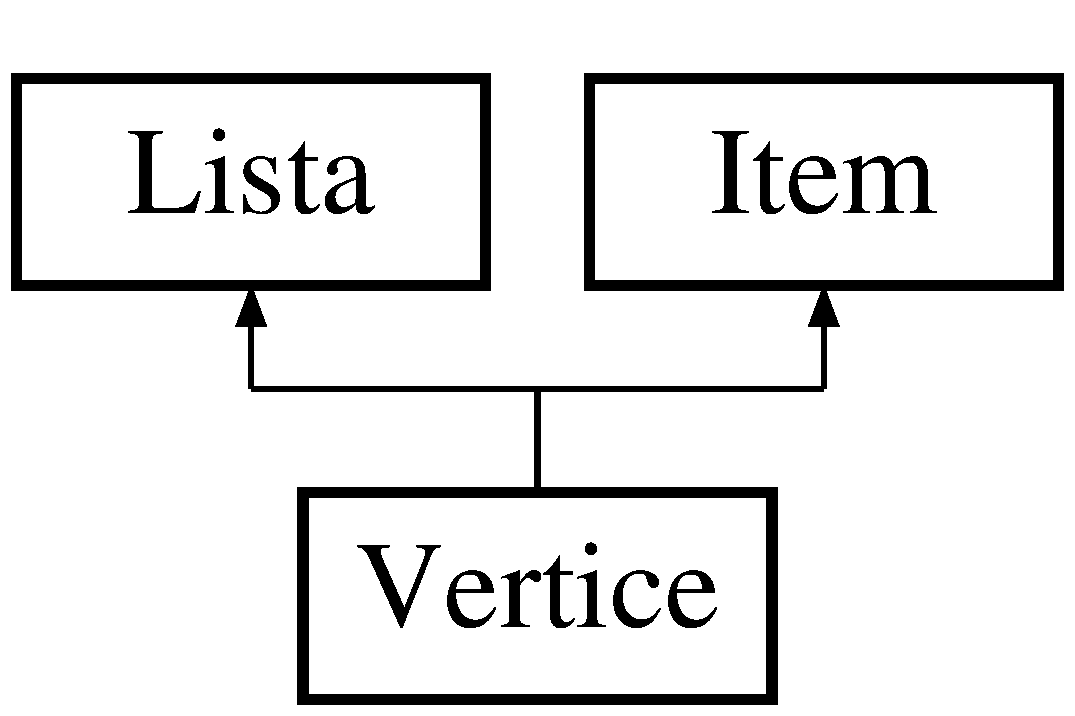
\includegraphics[height=2.000000cm]{class_vertice}
\end{center}
\end{figure}
\subsection*{Public Member Functions}
\begin{DoxyCompactItemize}
\item 
\hyperlink{class_vertice_a230fd673ca5c794ff5d4fb53dd98ca7b}{Vertice} (int Id)
\item 
\hyperlink{class_vertice_ae231694dc3ff35959b5b20b879b4678a}{$\sim$\-Vertice} ()
\begin{DoxyCompactList}\small\item\em Destrutor. \end{DoxyCompactList}\item 
bool \hyperlink{class_vertice_aa0003425b8eb7ec6c3d5cd915a88afbc}{foi\-Visitado} ()
\item 
void \hyperlink{class_vertice_aca656c6efc4478a597d0e2ced0d392e9}{seta\-Visitado} (bool vi)
\item 
int \hyperlink{class_vertice_abc05ac8e91788aa9fdd903bbbc6e37af}{pega\-Id} ()
\item 
int \hyperlink{class_vertice_a926f0ba5d1a1b202df2e91712fa3f3d0}{pega\-Grau} ()
\item 
void \hyperlink{class_vertice_a6d4a399b37a0126660fe73c7ba97654a}{adiciona\-Aresta} (int id\-\_\-destino)
\item 
void \hyperlink{class_vertice_acb35c8eb7a44fb79b2bbc3b77ac018ce}{adiciona\-Aresta} (int id\-\_\-destino, float peso)
\item 
void \hyperlink{class_vertice_a4024393ae653b1cc889780ae1801a152}{remove\-Aresta} ()
\item 
void \hyperlink{class_vertice_a3fd85d9c14304c70c0def1adb65b8fde}{set\-Particao} (int part)
\item 
int \hyperlink{class_vertice_a5de6dd2ebceaeca99f02c2cf8ec2f38d}{get\-Particao} ()
\item 
bool \hyperlink{class_vertice_a440a8735f0d7296bd9108951558bc30b}{remove\-Aresta} (int id)
\begin{DoxyCompactList}\small\item\em Remove aresta do \hyperlink{class_vertice}{Vertice} se encontra-\/la. \end{DoxyCompactList}\item 
bool \hyperlink{class_vertice_a6ec71f04fba51e1f7aab78fbe6fed820}{existe\-Aresta} (int id)
\begin{DoxyCompactList}\small\item\em Verifica se a aresta com id esxite. \end{DoxyCompactList}\item 
\hyperlink{class_aresta}{Aresta} $\ast$ \hyperlink{class_vertice_a2c2ca06ce42e54a04097e47c619d85c5}{primeira\-Aresta} ()
\item 
\hyperlink{class_aresta}{Aresta} $\ast$ \hyperlink{class_vertice_a89d7b87a3a89a747cc6676ad0ec0d1c1}{proxima\-Aresta} ()
\item 
\hyperlink{class_aresta}{Aresta} $\ast$ \hyperlink{class_vertice_a4b1e41a091fbc9bca36d2c0f1f921def}{aresta\-Anterior} ()
\item 
\hyperlink{class_aresta}{Aresta} $\ast$ \hyperlink{class_vertice_a91342a38cb831d4d7b531698c120f1d2}{ultima\-Aresta} ()
\item 
\hyperlink{class_aresta}{Aresta} $\ast$ \hyperlink{class_vertice_a1f54ebe5c618bca5266c1b48dd40e7e5}{encontra\-Aresta} (int id)
\begin{DoxyCompactList}\small\item\em Encontra uma \hyperlink{class_aresta}{Aresta} para id no \hyperlink{class_vertice}{Vertice} v. \end{DoxyCompactList}\item 
float \hyperlink{class_vertice_a4581200c3fb68557fd46cd8a7a32924c}{pega\-Peso\-Aresta} (int id)
\begin{DoxyCompactList}\small\item\em Retorna o peso da aresta passado por parametro. \end{DoxyCompactList}\end{DoxyCompactItemize}
\subsection*{Additional Inherited Members}


\subsection{Constructor \& Destructor Documentation}
\hypertarget{class_vertice_a230fd673ca5c794ff5d4fb53dd98ca7b}{\index{Vertice@{Vertice}!Vertice@{Vertice}}
\index{Vertice@{Vertice}!Vertice@{Vertice}}
\subsubsection[{Vertice}]{\setlength{\rightskip}{0pt plus 5cm}Vertice\-::\-Vertice (
\begin{DoxyParamCaption}
\item[{int}]{Id}
\end{DoxyParamCaption}
)\hspace{0.3cm}{\ttfamily [inline]}}}\label{class_vertice_a230fd673ca5c794ff5d4fb53dd98ca7b}
\hypertarget{class_vertice_ae231694dc3ff35959b5b20b879b4678a}{\index{Vertice@{Vertice}!$\sim$\-Vertice@{$\sim$\-Vertice}}
\index{$\sim$\-Vertice@{$\sim$\-Vertice}!Vertice@{Vertice}}
\subsubsection[{$\sim$\-Vertice}]{\setlength{\rightskip}{0pt plus 5cm}Vertice\-::$\sim$\-Vertice (
\begin{DoxyParamCaption}
{}
\end{DoxyParamCaption}
)}}\label{class_vertice_ae231694dc3ff35959b5b20b879b4678a}


Destrutor. 



\subsection{Member Function Documentation}
\hypertarget{class_vertice_a6d4a399b37a0126660fe73c7ba97654a}{\index{Vertice@{Vertice}!adiciona\-Aresta@{adiciona\-Aresta}}
\index{adiciona\-Aresta@{adiciona\-Aresta}!Vertice@{Vertice}}
\subsubsection[{adiciona\-Aresta}]{\setlength{\rightskip}{0pt plus 5cm}void Vertice\-::adiciona\-Aresta (
\begin{DoxyParamCaption}
\item[{int}]{id\-\_\-destino}
\end{DoxyParamCaption}
)\hspace{0.3cm}{\ttfamily [inline]}}}\label{class_vertice_a6d4a399b37a0126660fe73c7ba97654a}
\hypertarget{class_vertice_acb35c8eb7a44fb79b2bbc3b77ac018ce}{\index{Vertice@{Vertice}!adiciona\-Aresta@{adiciona\-Aresta}}
\index{adiciona\-Aresta@{adiciona\-Aresta}!Vertice@{Vertice}}
\subsubsection[{adiciona\-Aresta}]{\setlength{\rightskip}{0pt plus 5cm}void Vertice\-::adiciona\-Aresta (
\begin{DoxyParamCaption}
\item[{int}]{id\-\_\-destino, }
\item[{float}]{peso}
\end{DoxyParamCaption}
)\hspace{0.3cm}{\ttfamily [inline]}}}\label{class_vertice_acb35c8eb7a44fb79b2bbc3b77ac018ce}
\hypertarget{class_vertice_a4b1e41a091fbc9bca36d2c0f1f921def}{\index{Vertice@{Vertice}!aresta\-Anterior@{aresta\-Anterior}}
\index{aresta\-Anterior@{aresta\-Anterior}!Vertice@{Vertice}}
\subsubsection[{aresta\-Anterior}]{\setlength{\rightskip}{0pt plus 5cm}{\bf Aresta}$\ast$ Vertice\-::aresta\-Anterior (
\begin{DoxyParamCaption}
{}
\end{DoxyParamCaption}
)\hspace{0.3cm}{\ttfamily [inline]}}}\label{class_vertice_a4b1e41a091fbc9bca36d2c0f1f921def}
\hypertarget{class_vertice_a1f54ebe5c618bca5266c1b48dd40e7e5}{\index{Vertice@{Vertice}!encontra\-Aresta@{encontra\-Aresta}}
\index{encontra\-Aresta@{encontra\-Aresta}!Vertice@{Vertice}}
\subsubsection[{encontra\-Aresta}]{\setlength{\rightskip}{0pt plus 5cm}{\bf Aresta} $\ast$ Vertice\-::encontra\-Aresta (
\begin{DoxyParamCaption}
\item[{int}]{id}
\end{DoxyParamCaption}
)}}\label{class_vertice_a1f54ebe5c618bca5266c1b48dd40e7e5}


Encontra uma \hyperlink{class_aresta}{Aresta} para id no \hyperlink{class_vertice}{Vertice} v. 


\begin{DoxyParams}{Parameters}
{\em int} & id \\
\hline
\end{DoxyParams}
\begin{DoxyReturn}{Returns}
Aresta$\ast$ 
\end{DoxyReturn}
\hypertarget{class_vertice_a6ec71f04fba51e1f7aab78fbe6fed820}{\index{Vertice@{Vertice}!existe\-Aresta@{existe\-Aresta}}
\index{existe\-Aresta@{existe\-Aresta}!Vertice@{Vertice}}
\subsubsection[{existe\-Aresta}]{\setlength{\rightskip}{0pt plus 5cm}bool Vertice\-::existe\-Aresta (
\begin{DoxyParamCaption}
\item[{int}]{id}
\end{DoxyParamCaption}
)}}\label{class_vertice_a6ec71f04fba51e1f7aab78fbe6fed820}


Verifica se a aresta com id esxite. 


\begin{DoxyParams}{Parameters}
{\em int} & id \\
\hline
\end{DoxyParams}
\begin{DoxyReturn}{Returns}
bool 
\end{DoxyReturn}
\hypertarget{class_vertice_aa0003425b8eb7ec6c3d5cd915a88afbc}{\index{Vertice@{Vertice}!foi\-Visitado@{foi\-Visitado}}
\index{foi\-Visitado@{foi\-Visitado}!Vertice@{Vertice}}
\subsubsection[{foi\-Visitado}]{\setlength{\rightskip}{0pt plus 5cm}bool Vertice\-::foi\-Visitado (
\begin{DoxyParamCaption}
{}
\end{DoxyParamCaption}
)\hspace{0.3cm}{\ttfamily [inline]}}}\label{class_vertice_aa0003425b8eb7ec6c3d5cd915a88afbc}
\hypertarget{class_vertice_a5de6dd2ebceaeca99f02c2cf8ec2f38d}{\index{Vertice@{Vertice}!get\-Particao@{get\-Particao}}
\index{get\-Particao@{get\-Particao}!Vertice@{Vertice}}
\subsubsection[{get\-Particao}]{\setlength{\rightskip}{0pt plus 5cm}int Vertice\-::get\-Particao (
\begin{DoxyParamCaption}
{}
\end{DoxyParamCaption}
)\hspace{0.3cm}{\ttfamily [inline]}}}\label{class_vertice_a5de6dd2ebceaeca99f02c2cf8ec2f38d}
\hypertarget{class_vertice_a926f0ba5d1a1b202df2e91712fa3f3d0}{\index{Vertice@{Vertice}!pega\-Grau@{pega\-Grau}}
\index{pega\-Grau@{pega\-Grau}!Vertice@{Vertice}}
\subsubsection[{pega\-Grau}]{\setlength{\rightskip}{0pt plus 5cm}int Vertice\-::pega\-Grau (
\begin{DoxyParamCaption}
{}
\end{DoxyParamCaption}
)\hspace{0.3cm}{\ttfamily [inline]}}}\label{class_vertice_a926f0ba5d1a1b202df2e91712fa3f3d0}
\hypertarget{class_vertice_abc05ac8e91788aa9fdd903bbbc6e37af}{\index{Vertice@{Vertice}!pega\-Id@{pega\-Id}}
\index{pega\-Id@{pega\-Id}!Vertice@{Vertice}}
\subsubsection[{pega\-Id}]{\setlength{\rightskip}{0pt plus 5cm}int Vertice\-::pega\-Id (
\begin{DoxyParamCaption}
{}
\end{DoxyParamCaption}
)\hspace{0.3cm}{\ttfamily [inline]}}}\label{class_vertice_abc05ac8e91788aa9fdd903bbbc6e37af}
\hypertarget{class_vertice_a4581200c3fb68557fd46cd8a7a32924c}{\index{Vertice@{Vertice}!pega\-Peso\-Aresta@{pega\-Peso\-Aresta}}
\index{pega\-Peso\-Aresta@{pega\-Peso\-Aresta}!Vertice@{Vertice}}
\subsubsection[{pega\-Peso\-Aresta}]{\setlength{\rightskip}{0pt plus 5cm}float Vertice\-::pega\-Peso\-Aresta (
\begin{DoxyParamCaption}
\item[{int}]{id}
\end{DoxyParamCaption}
)}}\label{class_vertice_a4581200c3fb68557fd46cd8a7a32924c}


Retorna o peso da aresta passado por parametro. 


\begin{DoxyParams}{Parameters}
{\em int} & id \\
\hline
\end{DoxyParams}
\begin{DoxyReturn}{Returns}
float 
\end{DoxyReturn}
\hypertarget{class_vertice_a2c2ca06ce42e54a04097e47c619d85c5}{\index{Vertice@{Vertice}!primeira\-Aresta@{primeira\-Aresta}}
\index{primeira\-Aresta@{primeira\-Aresta}!Vertice@{Vertice}}
\subsubsection[{primeira\-Aresta}]{\setlength{\rightskip}{0pt plus 5cm}{\bf Aresta}$\ast$ Vertice\-::primeira\-Aresta (
\begin{DoxyParamCaption}
{}
\end{DoxyParamCaption}
)\hspace{0.3cm}{\ttfamily [inline]}}}\label{class_vertice_a2c2ca06ce42e54a04097e47c619d85c5}
\hypertarget{class_vertice_a89d7b87a3a89a747cc6676ad0ec0d1c1}{\index{Vertice@{Vertice}!proxima\-Aresta@{proxima\-Aresta}}
\index{proxima\-Aresta@{proxima\-Aresta}!Vertice@{Vertice}}
\subsubsection[{proxima\-Aresta}]{\setlength{\rightskip}{0pt plus 5cm}{\bf Aresta}$\ast$ Vertice\-::proxima\-Aresta (
\begin{DoxyParamCaption}
{}
\end{DoxyParamCaption}
)\hspace{0.3cm}{\ttfamily [inline]}}}\label{class_vertice_a89d7b87a3a89a747cc6676ad0ec0d1c1}
\hypertarget{class_vertice_a4024393ae653b1cc889780ae1801a152}{\index{Vertice@{Vertice}!remove\-Aresta@{remove\-Aresta}}
\index{remove\-Aresta@{remove\-Aresta}!Vertice@{Vertice}}
\subsubsection[{remove\-Aresta}]{\setlength{\rightskip}{0pt plus 5cm}void Vertice\-::remove\-Aresta (
\begin{DoxyParamCaption}
{}
\end{DoxyParamCaption}
)\hspace{0.3cm}{\ttfamily [inline]}}}\label{class_vertice_a4024393ae653b1cc889780ae1801a152}
\hypertarget{class_vertice_a440a8735f0d7296bd9108951558bc30b}{\index{Vertice@{Vertice}!remove\-Aresta@{remove\-Aresta}}
\index{remove\-Aresta@{remove\-Aresta}!Vertice@{Vertice}}
\subsubsection[{remove\-Aresta}]{\setlength{\rightskip}{0pt plus 5cm}bool Vertice\-::remove\-Aresta (
\begin{DoxyParamCaption}
\item[{int}]{id}
\end{DoxyParamCaption}
)}}\label{class_vertice_a440a8735f0d7296bd9108951558bc30b}


Remove aresta do \hyperlink{class_vertice}{Vertice} se encontra-\/la. 


\begin{DoxyParams}{Parameters}
{\em int} & id \\
\hline
\end{DoxyParams}
\begin{DoxyReturn}{Returns}
bool 
\end{DoxyReturn}
\hypertarget{class_vertice_aca656c6efc4478a597d0e2ced0d392e9}{\index{Vertice@{Vertice}!seta\-Visitado@{seta\-Visitado}}
\index{seta\-Visitado@{seta\-Visitado}!Vertice@{Vertice}}
\subsubsection[{seta\-Visitado}]{\setlength{\rightskip}{0pt plus 5cm}void Vertice\-::seta\-Visitado (
\begin{DoxyParamCaption}
\item[{bool}]{vi}
\end{DoxyParamCaption}
)\hspace{0.3cm}{\ttfamily [inline]}}}\label{class_vertice_aca656c6efc4478a597d0e2ced0d392e9}
\hypertarget{class_vertice_a3fd85d9c14304c70c0def1adb65b8fde}{\index{Vertice@{Vertice}!set\-Particao@{set\-Particao}}
\index{set\-Particao@{set\-Particao}!Vertice@{Vertice}}
\subsubsection[{set\-Particao}]{\setlength{\rightskip}{0pt plus 5cm}void Vertice\-::set\-Particao (
\begin{DoxyParamCaption}
\item[{int}]{part}
\end{DoxyParamCaption}
)\hspace{0.3cm}{\ttfamily [inline]}}}\label{class_vertice_a3fd85d9c14304c70c0def1adb65b8fde}
\hypertarget{class_vertice_a91342a38cb831d4d7b531698c120f1d2}{\index{Vertice@{Vertice}!ultima\-Aresta@{ultima\-Aresta}}
\index{ultima\-Aresta@{ultima\-Aresta}!Vertice@{Vertice}}
\subsubsection[{ultima\-Aresta}]{\setlength{\rightskip}{0pt plus 5cm}{\bf Aresta}$\ast$ Vertice\-::ultima\-Aresta (
\begin{DoxyParamCaption}
{}
\end{DoxyParamCaption}
)\hspace{0.3cm}{\ttfamily [inline]}}}\label{class_vertice_a91342a38cb831d4d7b531698c120f1d2}


The documentation for this class was generated from the following files\-:\begin{DoxyCompactItemize}
\item 
\hyperlink{_grafo_8h}{Grafo.\-h}\item 
\hyperlink{_grafo_8cpp}{Grafo.\-cpp}\end{DoxyCompactItemize}

\chapter{File Documentation}
\hypertarget{_grafo_8cpp}{\section{Grafo.\-cpp File Reference}
\label{_grafo_8cpp}\index{Grafo.\-cpp@{Grafo.\-cpp}}
}
{\ttfamily \#include \char`\"{}Grafo.\-h\char`\"{}}\\*
{\ttfamily \#include $<$iostream$>$}\\*
{\ttfamily \#include $<$vector$>$}\\*
{\ttfamily \#include $<$stdio.\-h$>$}\\*
{\ttfamily \#include $<$stdlib.\-h$>$}\\*
{\ttfamily \#include $<$limits$>$}\\*
{\ttfamily \#include $<$algorithm$>$}\\*
{\ttfamily \#include $<$string.\-h$>$}\\*
{\ttfamily \#include $<$list$>$}\\*
{\ttfamily \#include $<$queue$>$}\\*
{\ttfamily \#include $<$functional$>$}\\*
\subsection*{Macros}
\begin{DoxyCompactItemize}
\item 
\#define \hyperlink{_grafo_8cpp_af076440f216f5a40a11563e489f04932}{I\-N\-F\-I\-N\-I\-T\-O}~999999
\end{DoxyCompactItemize}


\subsection{Macro Definition Documentation}
\hypertarget{_grafo_8cpp_af076440f216f5a40a11563e489f04932}{\index{Grafo.\-cpp@{Grafo.\-cpp}!I\-N\-F\-I\-N\-I\-T\-O@{I\-N\-F\-I\-N\-I\-T\-O}}
\index{I\-N\-F\-I\-N\-I\-T\-O@{I\-N\-F\-I\-N\-I\-T\-O}!Grafo.cpp@{Grafo.\-cpp}}
\subsubsection[{I\-N\-F\-I\-N\-I\-T\-O}]{\setlength{\rightskip}{0pt plus 5cm}\#define I\-N\-F\-I\-N\-I\-T\-O~999999}}\label{_grafo_8cpp_af076440f216f5a40a11563e489f04932}
\hyperlink{_grafo_8cpp}{Grafo.\-cpp} 
\hypertarget{_grafo_8h}{\section{Grafo.\-h File Reference}
\label{_grafo_8h}\index{Grafo.\-h@{Grafo.\-h}}
}
{\ttfamily \#include \char`\"{}Lista.\-h\char`\"{}}\\*
{\ttfamily \#include $<$iostream$>$}\\*
{\ttfamily \#include $<$vector$>$}\\*
\subsection*{Classes}
\begin{DoxyCompactItemize}
\item 
class \hyperlink{class_aresta}{Aresta}
\item 
class \hyperlink{class_vertice}{Vertice}
\item 
class \hyperlink{class_grafo}{Grafo}
\end{DoxyCompactItemize}

\hypertarget{_leitura_gravacao_8cpp}{\section{Leitura\-Gravacao.\-cpp File Reference}
\label{_leitura_gravacao_8cpp}\index{Leitura\-Gravacao.\-cpp@{Leitura\-Gravacao.\-cpp}}
}
{\ttfamily \#include \char`\"{}Leitura\-Gravacao.\-h\char`\"{}}\\*
{\ttfamily \#include \char`\"{}Grafo.\-h\char`\"{}}\\*
{\ttfamily \#include $<$iostream$>$}\\*
{\ttfamily \#include $<$fstream$>$}\\*
{\ttfamily \#include $<$vector$>$}\\*
{\ttfamily \#include $<$string.\-h$>$}\\*
{\ttfamily \#include $<$cstdlib$>$}\\*

\hypertarget{_leitura_gravacao_8h}{\section{Leitura\-Gravacao.\-h File Reference}
\label{_leitura_gravacao_8h}\index{Leitura\-Gravacao.\-h@{Leitura\-Gravacao.\-h}}
}
{\ttfamily \#include $<$iostream$>$}\\*
{\ttfamily \#include $<$fstream$>$}\\*
{\ttfamily \#include $<$vector$>$}\\*
{\ttfamily \#include $<$string$>$}\\*
{\ttfamily \#include $<$cstdlib$>$}\\*
{\ttfamily \#include \char`\"{}Grafo.\-h\char`\"{}}\\*
\subsection*{Classes}
\begin{DoxyCompactItemize}
\item 
class \hyperlink{class_leitura_gravacao}{Leitura\-Gravacao}
\end{DoxyCompactItemize}

\hypertarget{_lista_8cpp}{\section{Lista.\-cpp File Reference}
\label{_lista_8cpp}\index{Lista.\-cpp@{Lista.\-cpp}}
}
{\ttfamily \#include \char`\"{}Lista.\-h\char`\"{}}\\*
{\ttfamily \#include $<$iostream$>$}\\*

\hypertarget{_lista_8h}{\section{Lista.\-h File Reference}
\label{_lista_8h}\index{Lista.\-h@{Lista.\-h}}
}
\subsection*{Classes}
\begin{DoxyCompactItemize}
\item 
class \hyperlink{class_item}{Item}
\item 
class \hyperlink{class_lista}{Lista}
\end{DoxyCompactItemize}

\hypertarget{main_8cpp}{\section{main.\-cpp File Reference}
\label{main_8cpp}\index{main.\-cpp@{main.\-cpp}}
}
{\ttfamily \#include $<$iostream$>$}\\*
{\ttfamily \#include $<$string.\-h$>$}\\*
{\ttfamily \#include \char`\"{}Lista.\-h\char`\"{}}\\*
{\ttfamily \#include \char`\"{}Grafo.\-h\char`\"{}}\\*
{\ttfamily \#include \char`\"{}Leitura\-Gravacao.\-h\char`\"{}}\\*
{\ttfamily \#include $<$algorithm$>$}\\*
\subsection*{Macros}
\begin{DoxyCompactItemize}
\item 
\#define \hyperlink{main_8cpp_a0fced60795fab0adc9583ccdaf0a24d7}{Tex\-\_\-\-Arquivo}~100
\end{DoxyCompactItemize}
\subsection*{Functions}
\begin{DoxyCompactItemize}
\item 
int \hyperlink{main_8cpp_ae66f6b31b5ad750f1fe042a706a4e3d4}{main} ()
\end{DoxyCompactItemize}


\subsection{Macro Definition Documentation}
\hypertarget{main_8cpp_a0fced60795fab0adc9583ccdaf0a24d7}{\index{main.\-cpp@{main.\-cpp}!Tex\-\_\-\-Arquivo@{Tex\-\_\-\-Arquivo}}
\index{Tex\-\_\-\-Arquivo@{Tex\-\_\-\-Arquivo}!main.cpp@{main.\-cpp}}
\subsubsection[{Tex\-\_\-\-Arquivo}]{\setlength{\rightskip}{0pt plus 5cm}\#define Tex\-\_\-\-Arquivo~100}}\label{main_8cpp_a0fced60795fab0adc9583ccdaf0a24d7}


\subsection{Function Documentation}
\hypertarget{main_8cpp_ae66f6b31b5ad750f1fe042a706a4e3d4}{\index{main.\-cpp@{main.\-cpp}!main@{main}}
\index{main@{main}!main.cpp@{main.\-cpp}}
\subsubsection[{main}]{\setlength{\rightskip}{0pt plus 5cm}int main (
\begin{DoxyParamCaption}
{}
\end{DoxyParamCaption}
)}}\label{main_8cpp_ae66f6b31b5ad750f1fe042a706a4e3d4}

%--- End generated contents ---

% Index
\newpage
\phantomsection
\addcontentsline{toc}{chapter}{Index}
\printindex

\end{document}
